\chapter{Component And Connector Views}

\begin{justify}
    Given that a comprehensive Components and Connectors (C\&C) view of the entire system could prove overly dense and complex for detailed analysis, this chapter will instead present a series of focused views. These views are specifically tailored to illustrate the architectural components and their interconnections pertaining to the system's principal use cases.
\end{justify}

\section{General Details}
Some components are repeated in subsequent paragraphs and share common details and functionalities:

\begin{enumerate}
    \item \label{def:GenDetailsOrchestrator} \textbf{\hyperref[def:Orchestrator]{Orchestrator}:} This service acts as the API Gateway for the PeerFlow system. 
    \begin{itemize}
        \item \textbf{IAPIGateway interface - Entrypoint:} It receives HTTP requests from the Web Application and interacts with components of the PeerFlow system to accomplish the requested task.

        \item \textbf{Authorization Enforcement:} The Orchestrator is capable of verifying the JWT included in the requests it receives by using the public key of the  \hyperref[def:AuthProfilingService]{Auth \& Profiling Service}. It stores the public key in a local cache with a predetermined TTL and refreshes it when the TTL expires.
    \end{itemize}

    \item \label{def:GenDetailsAuth} \textbf{\hyperref[def:AuthProfilingService]{Auth \& Profiling Service}:} This microservice is responsible for user authentication and profile management. 
    \begin{itemize}
        \item \textbf{IPublicKey interface - Asymmetric Signature verification:} This interface allows other services to request the public key that can be used to verify the signature of the JWTs.
        \item \textbf{Auth DB:} This is the dedicated database instance for the Auth \& Profiling Service. It stores user profiles and roles, accessed for authorization checks and to retrieve user(s) data.
    \end{itemize}

    \item \label{def:GenDetailsNotification} \textbf{\hyperref[def:NotificationService]{Notification Service}:} This service exposes a REST API that allows to send email notifications to the users of the system.
    \begin{itemize}
        \item  \textbf{INotification interface:} Receives \texttt{sendNotification()} calls from the \hyperref[def:Orchestrator]{Orchestrator} and dispaches email notifications to selected users.
    \end{itemize}

    \item \label{def:GenDetailsOtherServices}\textbf{Other Services:} This aggregated component represents domain-specific microservices within the PeerFlow system that are not specifically relevant in the view.
    \begin{itemize}
        \item \textbf{IOtherServicesAPI:} This interface is an abstraction and aggregates all the interface provided by the Other Services of the system, shown for completeness of the PeerFlow architecture.
    \end{itemize}
\end{enumerate}

\clearpage

\section{Authentication}

\begin{figure}[h]
    \centering
    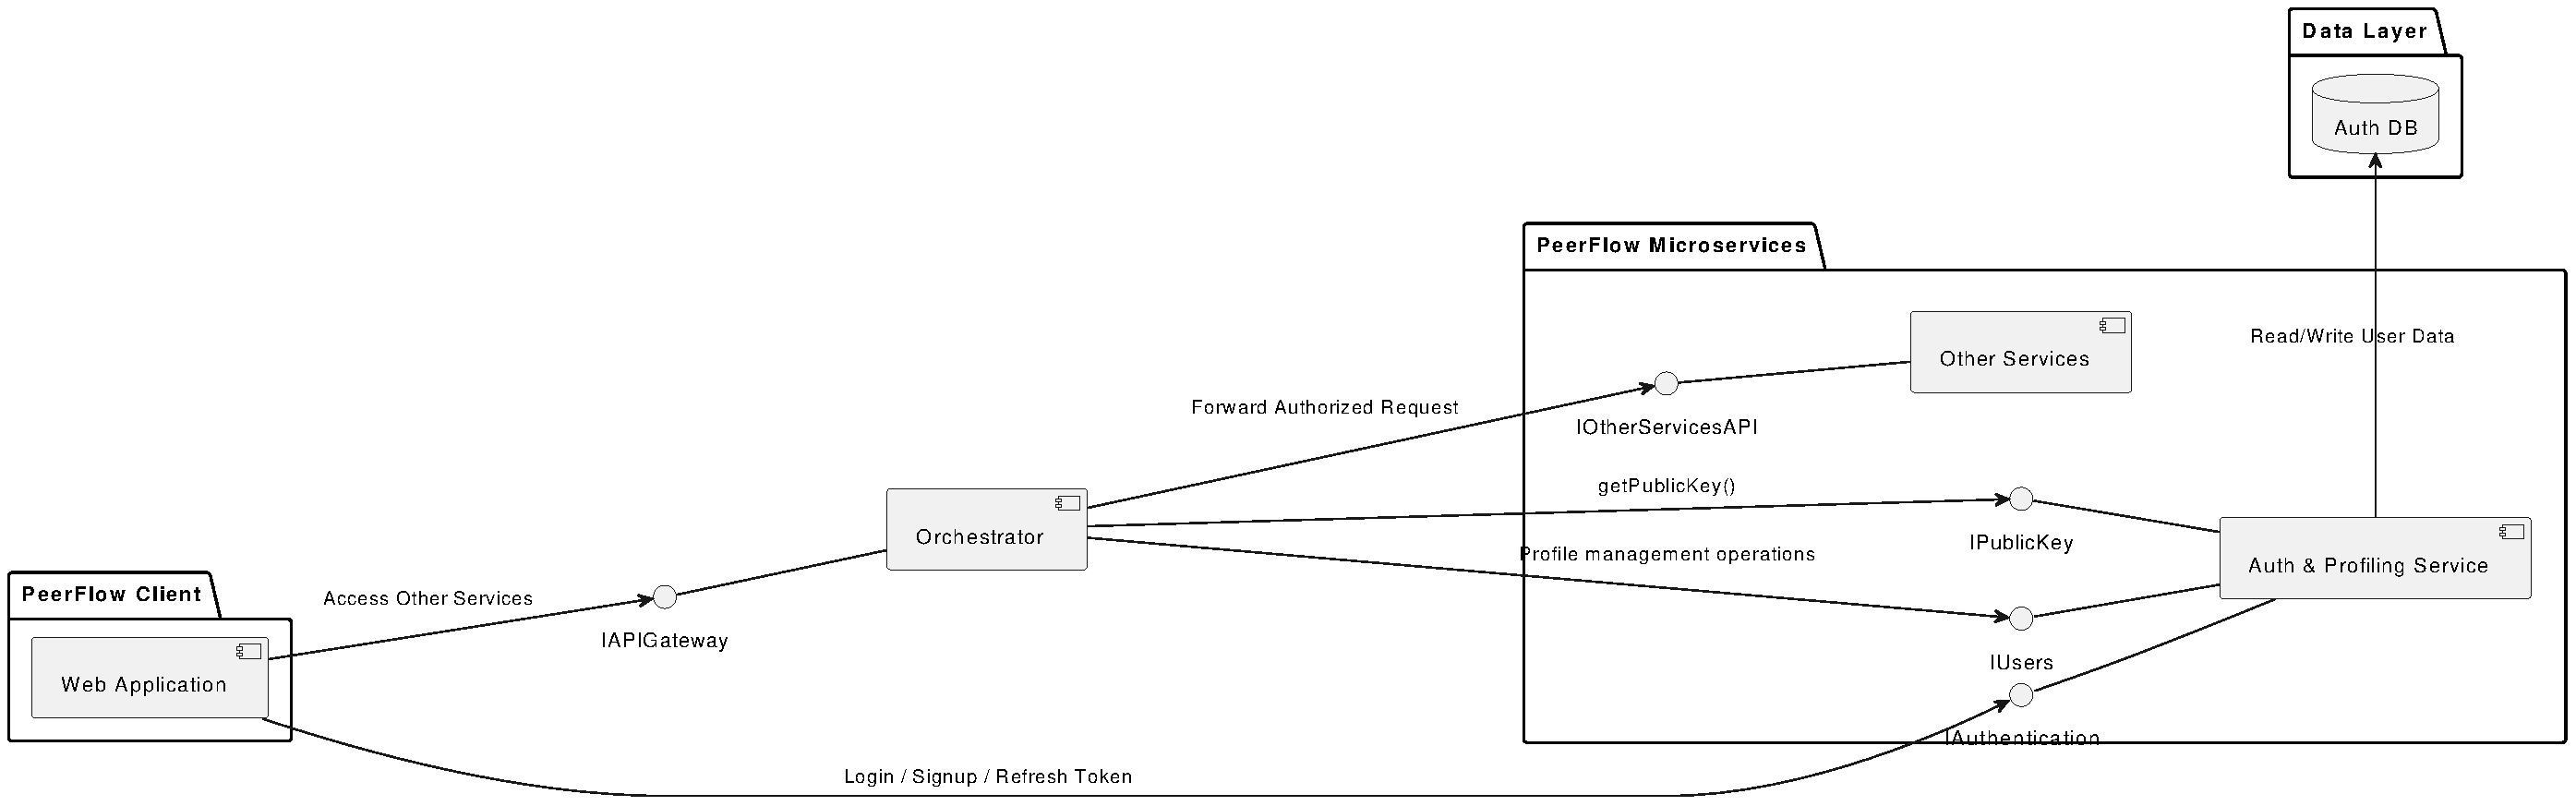
\includegraphics[width=0.9\linewidth]{Architettura/imgs/auth_cnc.pdf}
    \caption{C\&C view of the authentication process.}
    \label{fig:ccAuthentication}
\end{figure}

\subsection{Elements}

\begin{enumerate}
    \item \textbf{\hyperref[def:WebApplication]{Web Application}:} This is the client-side front-end application. It provides the user interface through which users can interact with the PeerFlow system’s microservices. 
    \begin{itemize}
        \item \textbf{User Login and Signup Form:} It presents a typical login/signup page and sends user credentials to the backend via the \hyperref[def:Orchestrator]{Orchestrator}. It also handles the storage and refreshing of JWT tokens.
    \end{itemize}
    \item \textbf{\hyperref[def:Orchestrator]{Orchestrator} \hyperref[def:GenDetailsOrchestrator]{[General Details]}:} This service acts as the API Gateway for the PeerFlow system. 
    
    \item \textbf{\hyperref[def:AuthProfilingService]{Auth \& Profiling Service} \hyperref[def:GenDetailsAuth]{[General Details]}:} This microservice is responsible for user authentication and profile management.  
    \begin{itemize}
        \item \textbf{IAuthentication interface - Authentication:} Allows the user to sign up, log in, obtain access and refresh JWTs, and refresh the access token.

        \item \textbf{IPublicKey interface - Public Key Discovery:} Provides an endpoint to retrieve the public key of the \hyperref[def:AuthProfilingService]{Auth \& Profiling Service}, which can be used to verify its signature on the JWTs. Each JWT is signed with \textbf{ES256} asymmetric signature algorithm, which allows other systems to verify the signature without interacting with \hyperref[def:AuthProfilingService]{Auth \& Profiling Service}.

        \item \textbf{IUsers interface:} Provides methods to execute CRUD operations on user profiles.
    \end{itemize}
    
    \item \textbf{Other Services \hyperref[def:GenDetailsOtherServices]{[General Details]}:} This aggregated component represents domain-specific microservices within the PeerFlow system that are not specifically relevant in the view.
\end{enumerate}


\clearpage
\subsection{Sequence Diagram}

\begin{figure}[h]
    \centering
    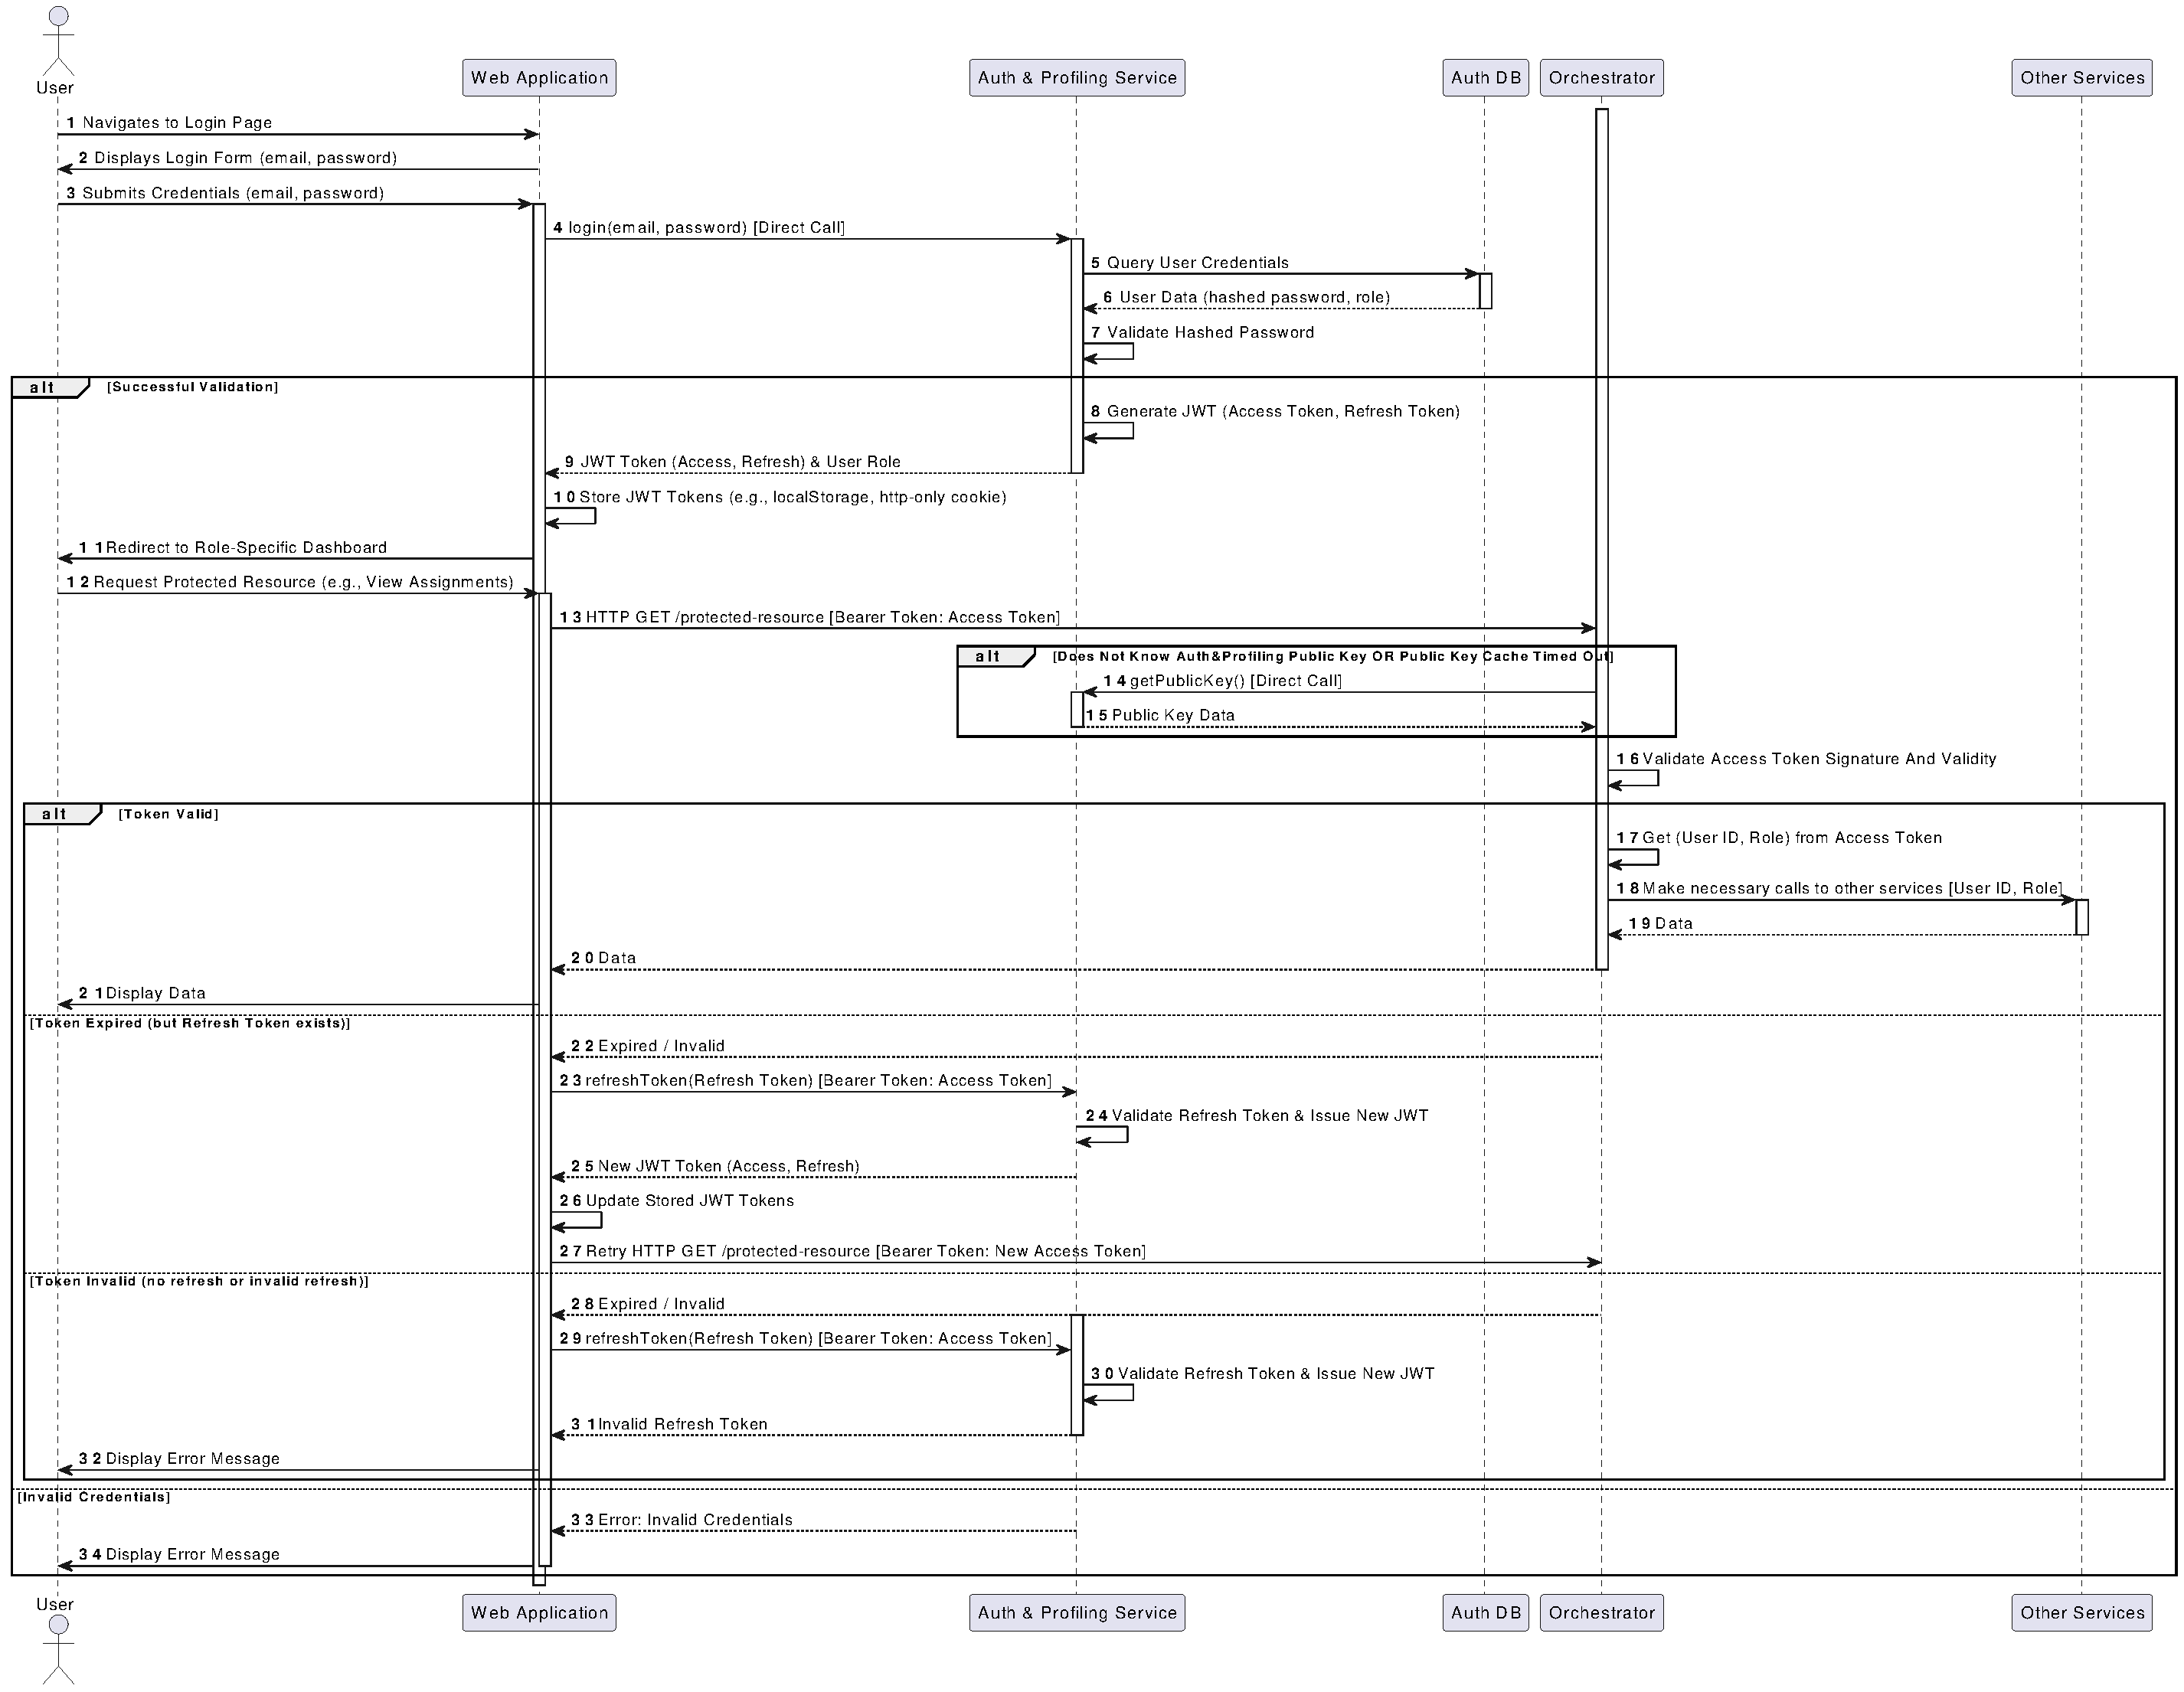
\includegraphics[width=0.9\linewidth]{Architettura/imgs/auth_seq.pdf}
    \caption{Sequence diagram of the authentication process.}
    \label{fig:seqAuthentication}
\end{figure}

\subsection{Rationale}

\begin{justify}
    The design choices for the Authentication Flow are justified by the core requirements of security, scalability, and maintainability inherent in a MOOC-like platform, with a specific interaction pattern for authentication:
\end{justify}
\begin{itemize}
    \item \textbf{Dedicated \hyperref[def:AuthProfilingService]{Auth \& Profiling Service} with Clear Interfaces:}
    \begin{itemize}
        \item \textbf{Direct Authentication (Login/Signup/Refresh):} The \hyperref[def:WebApplication]{Web Application} directly interacts with the \hyperref[def:AuthProfilingService]{Auth \& Profiling Service} for user login, signup, and JWT refresh operations. This direct interaction can be optimized for low latency during these critical initial user interactions. \req{FR-SYS-002} states "The system shall require users to authenticate before accessing role-specific functionalities" and \req{FR-SYS-003} states "The system shall allow new users (Students or Teachers) to sign up". The \hyperref[def:AuthProfilingService]{Auth \& Profiling Service} is responsible for handling the user credentials and generating the necessary JWT tokens.
        \item \textbf{Security:} Centralizing all authentication logic, user management, and JWT token handling within the \hyperref[def:AuthProfilingService]{Auth \& Profiling Service} ensures that security concerns are isolated and can be managed with specialized expertise and tooling. This aligns with the Security constraint that "The system must ensure the security of user data and submissions". Explicit interfaces (IAuthentication, IAuthorization, ITokenManagement) clearly define the contract for interactions, enhancing security and reducing potential vulnerabilities.
        \item \textbf{Scalability:} Authentication is a high-traffic operation, especially in MOOCs with a large number of concurrent users. Isolating this functionality allows the \hyperref[def:AuthProfilingService]{Auth \& Profiling Service} to be independently scaled horizontally (e.g., \req{QA-PE-4}: Increase in Registered Users specifies maintaining login response times with increased users) without affecting other services.
        \item \textbf{Maintainability:} Changes to authentication mechanisms (e.g., adding multi-factor authentication) or user profile fields (e.g., \req{QA-MO-01}: Modifying the Student Data Model) are confined to this service, minimizing impact on the rest of the system. The system must support two distinct user roles: Teacher and Student.
    \end{itemize}

    \item \textbf{\hyperref[def:Orchestrator]{Orchestrator} as an API Gateway Primarily for Authorization Enforcement and Routing to Other Services:}
    \begin{itemize}
        \item \textbf{Unified Entry Point (for non-Auth APIs):} While not handling initial authentication requests directly from \hyperref[def:WebApplication]{WebApp}, the \hyperref[def:Orchestrator]{Orchestrator} still serves as the single entry point for all client requests targeting the "Other Services". This simplifies the \hyperref[def:WebApplication]{Web Application}'s interaction model for subsequent authorized requests.
        
        \item \textbf{Security Enforcement (JWT Verification):} The \hyperref[def:Orchestrator]{Orchestrator}'s primary role in the authentication flow is to verify the JWTs (signed using \textbf{ES256} asymmetric signature algorithm) using the public key of the   \hyperref[def:AuthProfilingService]{Auth \& Profiling Service} before forwarding requests to Other Services. This makes the \hyperref[def:Orchestrator]{Orchestrator} a crucial authorization gate, ensuring that only authenticated and authorized requests reach the downstream services. This means individual microservices (Other Services) do not need to implement their own authorization logic, reducing duplication and potential security vulnerabilities. This also supports the requirement to "enforce access restrictions by granting access only to the system functionalities, data, and user interface views appropriate for the identified user role".
    \end{itemize}

    \item \textbf{Token-Based Authentication (JWT):}
    \begin{itemize}
        \item \textbf{Statelessness:} JWTs are stateless, meaning the server does not need to store session information. This is critical for horizontal scalability, as any instance of a service (both \hyperref[def:AuthProfilingService]{Auth \& Profiling Service} and \hyperref[def:Orchestrator]{Orchestrator} for verification) can validate the token without needing to access shared session state. This directly supports the need for horizontal scalability, high availability, and low latency for a large and highly variable number of users.
        \item \textbf{Decoupling:} JWTs, managed by the \hyperref[def:AuthProfilingService]{Auth \& Profiling Service} and validated by the \hyperref[def:Orchestrator]{Orchestrator}, allow for a clear separation of concerns between authentication issuance and authorization enforcement across different components.
    \end{itemize}

    \item \textbf{Dedicated Auth DB:}
    \begin{itemize}
        \item \textbf{Data Isolation:} The Auth DB is exclusively for the \hyperref[def:AuthProfilingService]{Auth \& Profiling Service}. This aligns with the microservices principle of "data ownership," ensuring that the \hyperref[def:AuthProfilingService]{Auth \& Profiling Service} has full control over its data schema and evolution.
        \item \textbf{Performance and Scalability:} This isolation allows the Auth DB to be optimized and scaled independently, which is crucial given the potential for a "gradual but significant increase in the number of active users, profile creation requests, and general platform interactions" and the need to support a "50\% increase in concurrent users".
    \end{itemize}
\end{itemize}

\section{Assignment Creation}

\begin{figure}[h]
    \centering
    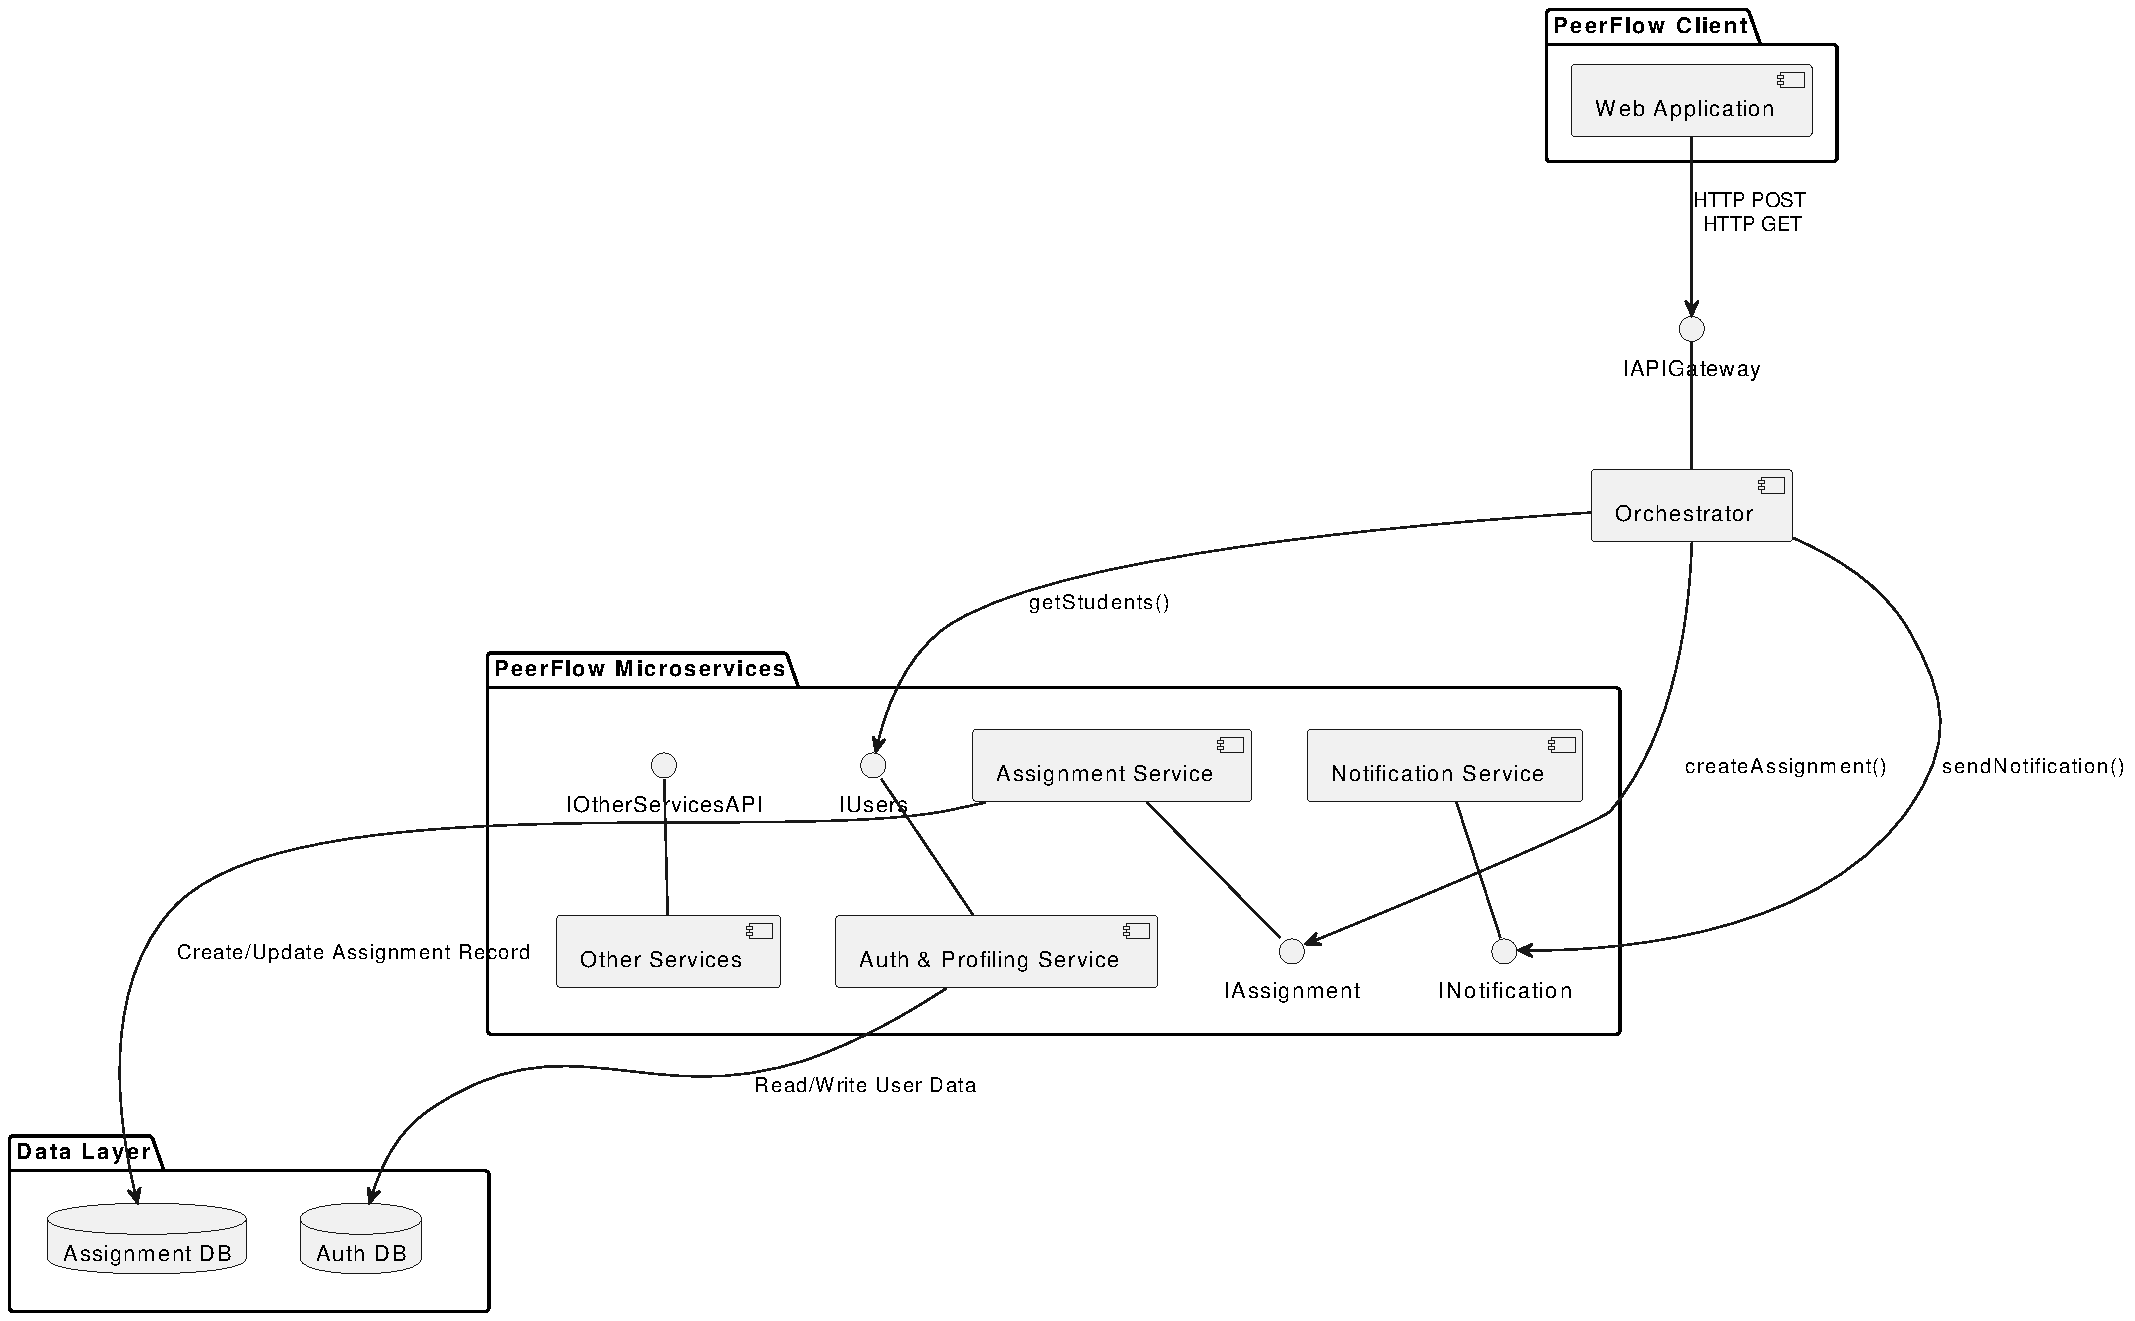
\includegraphics[width=0.9\linewidth]{Architettura/imgs/assign_create_cnc.pdf}
    \caption{C\&C view of the assignment creation process.}
    \label{fig:ccAssignmentCreation}
\end{figure}

\subsection{Elements}

\begin{enumerate}
    \item \textbf{\hyperref[def:WebApplication]{Web Application}:} This is the client-side front-end application. It provides the user interface through which users can interact with the PeerFlow system’s microservices. 
    \begin{itemize}
        \item \textbf{Assignment Creation Form:}  It provides the user interface through which teachers interact with the PeerFlow system. It presents the teacher with a form or page for creating a new assignment, allowing them to input details like the assignment name, description, deadline, and to select involved students. It initiates the HTTP \texttt{GET} request to retrieve the list of available students for selection. It sends the HTTP \texttt{POST} request containing all the assignment details, including the selected student IDs, to the \hyperref[def:Orchestrator]{Orchestrator}. 
    \end{itemize}

    \item \textbf{\hyperref[def:Orchestrator]{Orchestrator} \hyperref[def:GenDetailsOrchestrator]{[General Details]}:} This service acts as the API Gateway for the PeerFlow system.
    
    It is the single entry point for the \hyperref[def:WebApplication]{Web Application} to interact with most of the system's microservices.
    \begin{itemize}
       
        \item \textbf{Student Data Retrieval:} It calls the IUsers interface of the \hyperref[def:AuthProfilingService]{Auth \& Profiling Service} to fetch the list of registered students, which is then sent back to the \hyperref[def:WebApplication]{Web Application} for display in the assignment creation form.
        
        \item \textbf{Assignment Creation Orchestration:} It calls the IAssignment interface of the \hyperref[def:AssignmentService]{Assignment Service}, passing along all the assignment details provided by the teacher, including the selected list of involved student IDs.
        
        \item \textbf{Notification Trigger:} After the assignment is successfully created, it calls the INotification interface of the \hyperref[def:NotificationService]{Notification Service} to send email notifications to the newly involved students about the assignment.
    \end{itemize}
    
    \item \textbf{\hyperref[def:AuthProfilingService]{Auth \& Profiling Service} \hyperref[def:GenDetailsAuth]{[General Details]}:} This microservice is responsible for user authentication and profile management.
    
    \item \textbf{\hyperref[def:AssignmentService]{Assignment Service}:} This microservice manages the creation, modification, and viewing of assignments. 
    \begin{itemize}
        \item \textbf{IAssignment interface - Assignment Creation:}  It receives the calls by the \hyperref[def:Orchestrator]{Orchestrator} containing all the assignment details (name, description, deadline, and the list of involved student IDs). It validates the input (e.g., checking if the deadline is in the future) and generates a new assignment record, associating it with the creating teacher and the specified students in its dedicated data store.

        \item \textbf{IAssignment interface:} This interface also defines methods for general assignment management, such as viewing or modifying.

        \item \textbf{Assignment DB:} This is the dedicated database instance for the \hyperref[def:AssignmentService]{Assignment Service}. It stores all assignment-related data, such as the assignment's name, description, submission deadline, current status, and the list of involved student IDs.
    \end{itemize}
    
    \item \textbf{\hyperref[def:NotificationService]{Notification Service} \hyperref[def:GenDetailsNotification]{[General Details]}:} This service exposes a REST API that allows to send email notifications to the users of the system.
    
     \item \textbf{Other Services \hyperref[def:GenDetailsOtherServices]{[General Details]}:} This aggregated component represents domain-specific microservices within the PeerFlow system that are not specifically relevant in the view.
\end{enumerate}


\clearpage
\subsection{Sequence Diagram}

\begin{figure}[h]
    \centering
    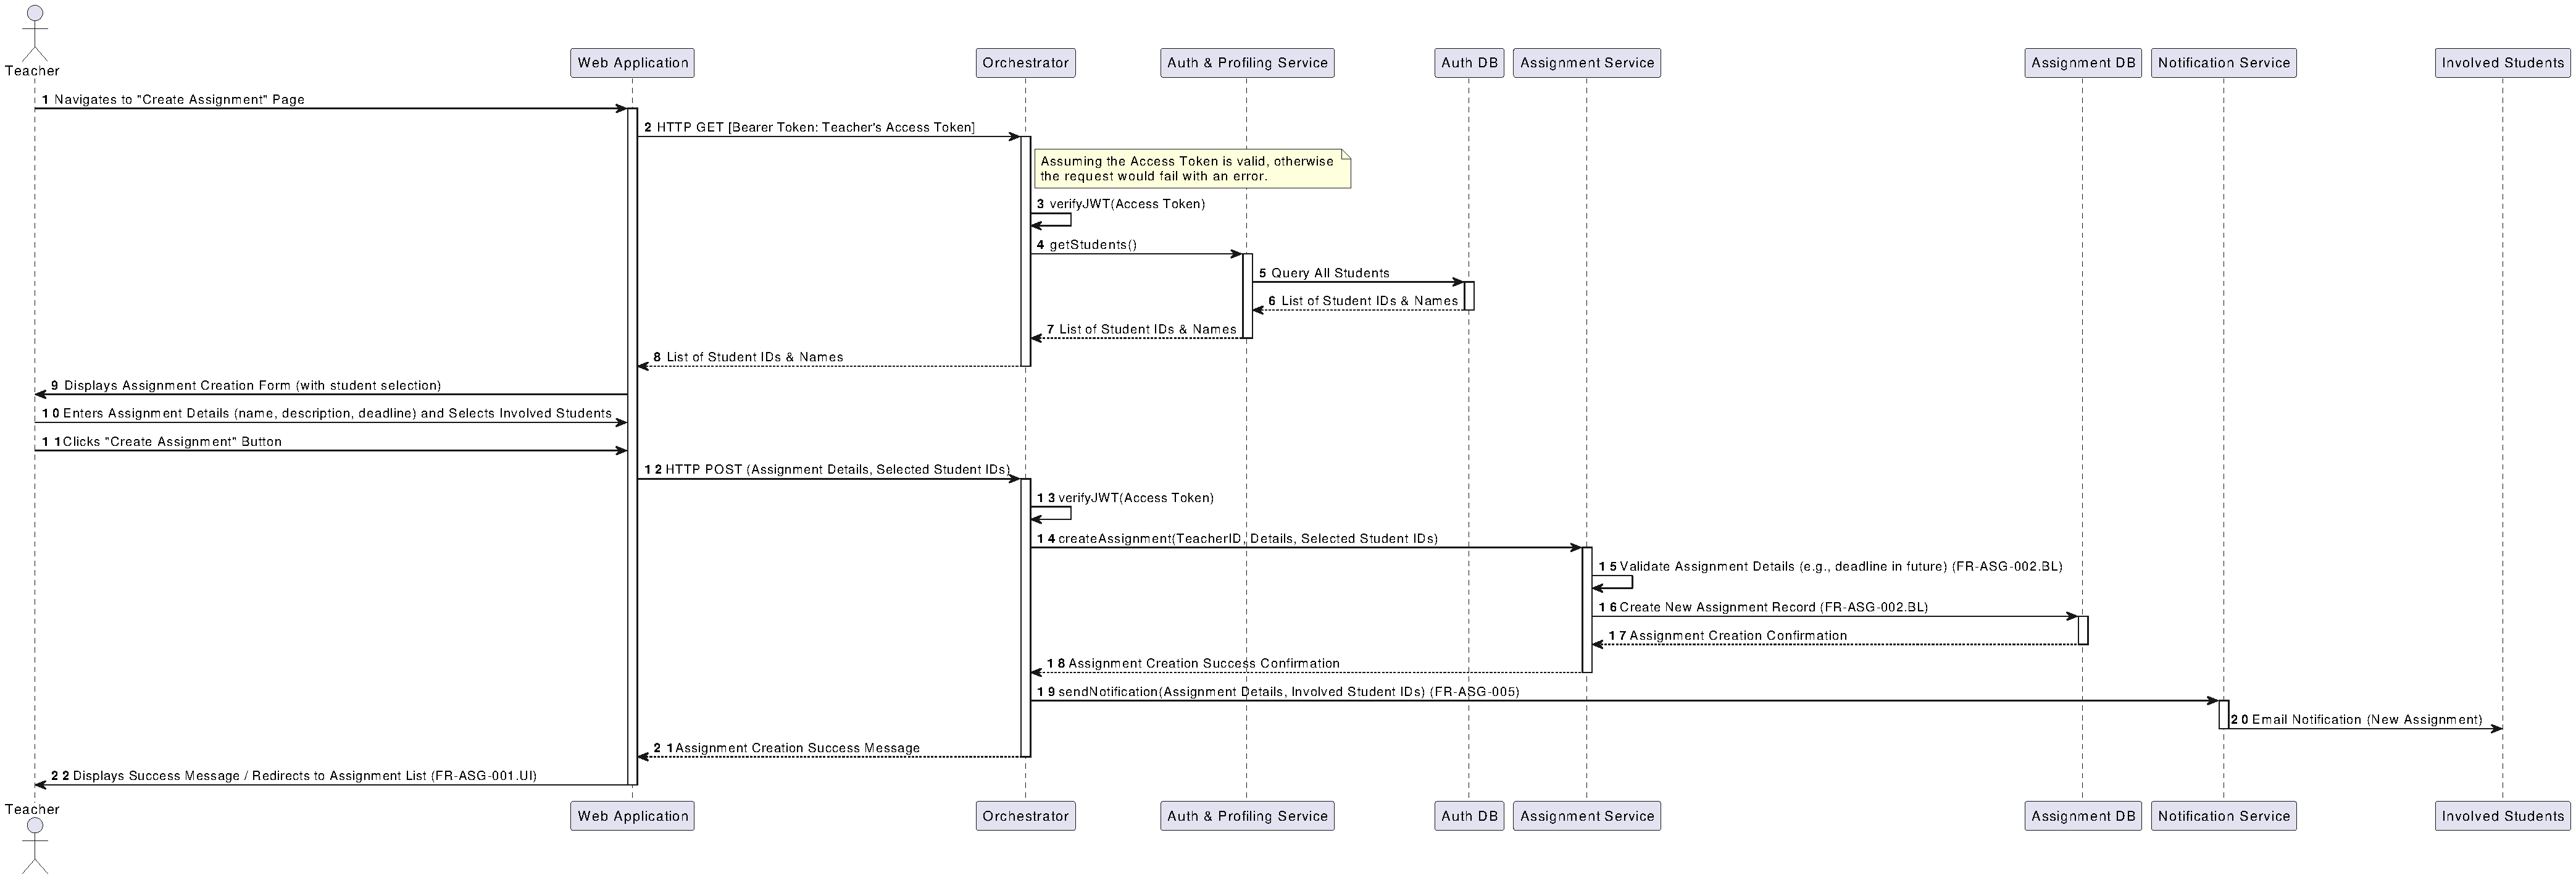
\includegraphics[width=0.9\linewidth]{Architettura/imgs/assign_create_seq.pdf}
    \caption{Sequence diagram of the assignment creation process.}
    \label{fig:seqAssignmentCreation}
\end{figure}

\subsection{Rationale}

\begin{itemize}
    \item \textbf{Teacher Role Enforcement and Authorization:}
    \begin{itemize}
        \item The flow ensures that only authenticated and authorized "Teachers" can create assignments. This is critical for data integrity and system security.
        \item The \hyperref[def:Orchestrator]{Orchestrator} acts as an API Gateway and is responsible for this initial authorization check by locally verifying JWT validity. This centralizes security enforcement, preventing other services from having to re-implement authentication/authorization logic for every request.
        \item The \hyperref[def:AuthProfilingService]{Auth \& Profiling Service} is the single source of truth for user roles and permissions.
    \end{itemize}
    \item \textbf{Efficient Student Involvement Management:}
    \begin{itemize}
        \item Teachers need to specify "involved students". The flow facilitates this by first allowing the \hyperref[def:WebApplication]{Web Application} to fetch a list of available students.
        \item By querying the IUsers interface of the \hyperref[def:AuthProfilingService]{Auth \& Profiling Service} via the \hyperref[def:Orchestrator]{Orchestrator}, the system ensures that the list of students is always up-to-date and consistent with the central user registry. This avoids data duplication if student data were cached or replicated in other services.
    \end{itemize}
    \item \textbf{Clear Separation of Concerns and Modularity:}
    \begin{itemize}
        \item The \hyperref[def:AssignmentService]{Assignment Service} is exclusively responsible for the business logic of creating assignments and managing assignment data (name, description, deadlines, associated students). This adheres to the microservices principle of single responsibility.
        \item Validation of assignment details, such as ensuring the "deadline is in the future", is handled directly by the \hyperref[def:AssignmentService]{Assignment Service}'s business logic.
        \item Changes to how assignments are created or their data structure can be implemented within the \hyperref[def:AssignmentService]{Assignment Service} without impacting other parts of the system, supporting the Modifiability non-functional requirement.
    \end{itemize}
    \item \textbf{Decoupled Notification System:}
    \begin{itemize}
        \item The requirement to "notify involved students (through email) when a new assignment is created" is handled by the \hyperref[def:NotificationService]{Notification Service}.
        \item The \hyperref[def:Orchestrator]{Orchestrator} triggers this notification after the \hyperref[def:AssignmentService]{Assignment Service} has successfully created the assignment. This loose coupling means the \hyperref[def:AssignmentService]{Assignment Service} does not need to know the specifics of email sending. It only needs to confirm the assignment's creation.
        \item The \hyperref[def:NotificationService]{Notification Service} can be independently scaled and can implement robust features like message queues and retry mechanisms to ensure reliable delivery, even if the primary assignment creation process is successful.
    \end{itemize}
    \item \textbf{Scalability and Performance:}
    \begin{itemize}
        \item The use of dedicated databases (Assignment DB and Auth DB) for each service ensures data autonomy and avoids contention that could arise from a shared database, contributing to better performance and scalability of the overall system.
    \end{itemize}
\end{itemize}
\begin{justify}
    This flow ensures that assignment creation is a secure, well-orchestrated, and maintainable process within the PeerFlow microservices ecosystem.
\end{justify}

\clearpage

\section{Assignment Submission}

\begin{figure}[h]
    \centering
    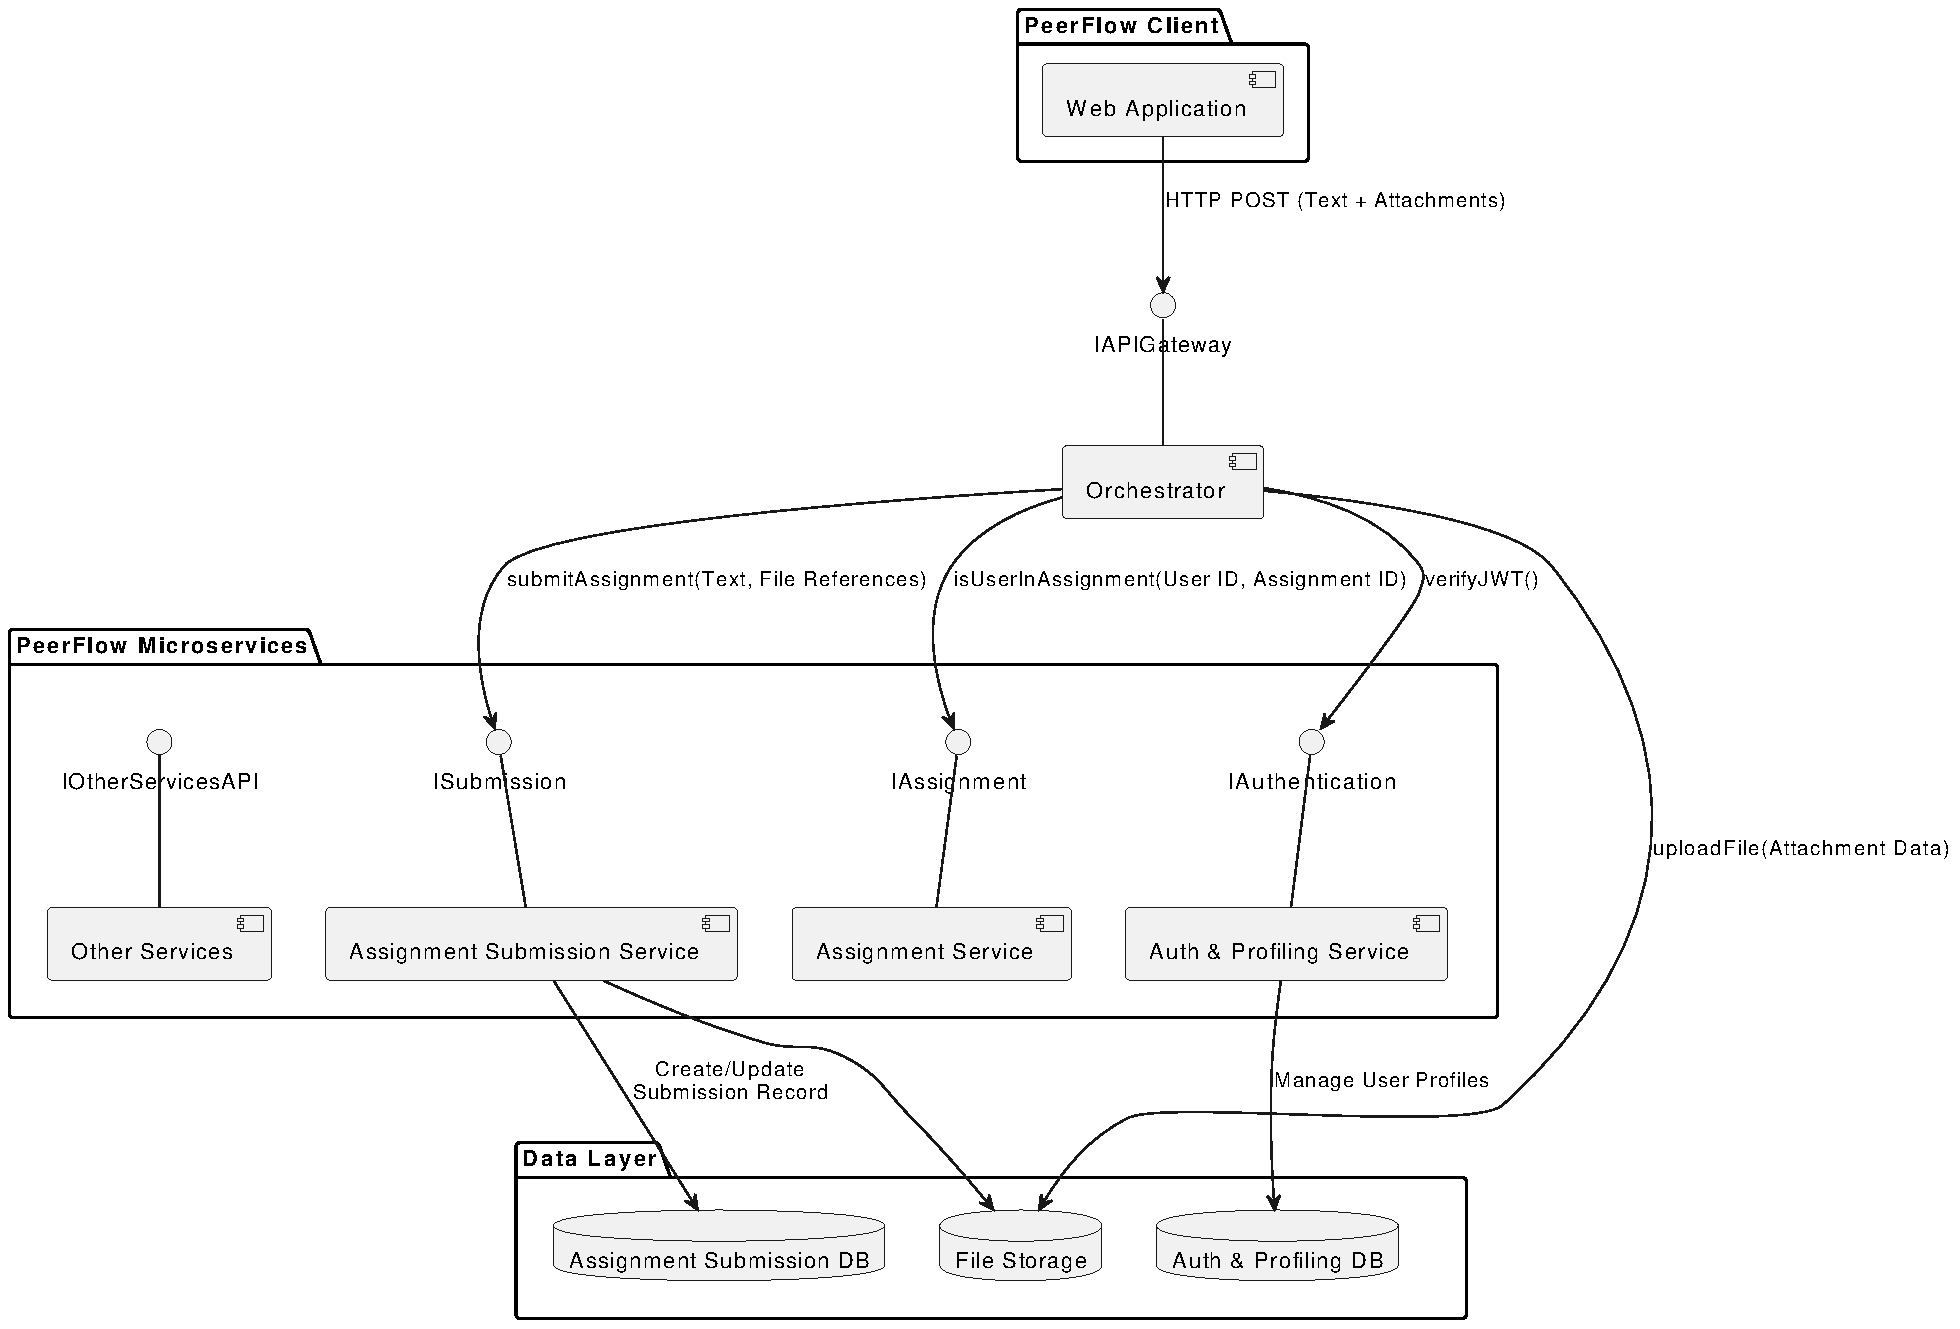
\includegraphics[width=0.9\linewidth]{Architettura/imgs/assign_submission_cnc.pdf}
    \caption{C\&C view of the assignment submission process.}
    \label{fig:ccAssignmentSubmission}
\end{figure}

\subsection{Elements}

\begin{enumerate}
    \item \textbf{\hyperref[def:WebApplication]{Web Application}:} This is the client-side front-end application. It provides the user interface through which users can interact with the PeerFlow system’s microservices.
    \begin{itemize}
        \item \textbf{Assignment Submission Form:} It shows a submission interface for an assignment, allowing the students to input textual content and (optionally) to upload file attachments (PDF, TXT, JPG). It sends the HTTP \texttt{POST} request, containing both the textual input and the file attachment data, to the \hyperref[def:Orchestrator]{Orchestrator}.
    \end{itemize}
    \item \textbf{\hyperref[def:Orchestrator]{Orchestrator} \hyperref[def:GenDetailsOrchestrator]{[General Details]}:} This service acts as the API Gateway for the PeerFlow system. It is the central coordinator for the submission flow.
    \begin{itemize}
        \item \textbf{File Handling Optimization:} The \hyperref[def:Orchestrator]{Orchestrator} directly calls the \texttt{uploadFile()} operation to upload files on the FileStorageDB (representing the \hyperref[def:FileStorageService]{File Storage Service}'s functionality). This allows to bypass the file transfer through the \hyperref[def:AssignmentSubmissionService]{Assignment Submission Service}.
        \item \textbf{Reference Passing:} After successfully uploading files and obtaining file references (e.g., URLs or unique IDs) from the FileStorageDB, the \hyperref[def:Orchestrator]{Orchestrator} calls the ISubmission interface of the \hyperref[def:AssignmentSubmissionService]{Assignment Submission Service}, finally registering the submission.
    \end{itemize}
    
    \item \textbf{\hyperref[def:AuthProfilingService]{Auth \& Profiling Service} \hyperref[def:GenDetailsAuth]{[General Details]}:} This microservice is responsible for user authentication and profile management.

    \item \textbf{\hyperref[def:AssignmentService]{Assignment Service}:} This microservice manages the creation, modification, and viewing of assignments.
    \begin{itemize}
        \item \textbf{IAssignment interface - Assignment List}: This interface allows the orchestrator to check if the student is assigned and allowed to send a submission.
    \end{itemize}

    \item \textbf{\hyperref[def:AssignmentSubmissionService]{Assignment Submission Service}:} This microservice handles the processing and recording of student submissions. 
    \begin{itemize}
        \item \textbf{ISubmission interface:} It receives \texttt{submitAssignment()} calls from the \hyperref[def:Orchestrator]{Orchestrator}. It processes the textual content and the file references received from the \hyperref[def:Orchestrator]{Orchestrator}. It performs business logic validations (e.g., ensuring submission is before the deadline). It registers the text, file references, and submission timestamp in its dedicated Assignment Submission DB.
        
        \item \textbf{Assignment Submission DB:} This is the dedicated database instance for the \hyperref[def:AssignmentSubmissionService]{Assignment Submission Service}. It stores submission metadata, including the textual content of the submission, the file references obtained from FileStorageDB, the student's ID, the assignment ID, and the submission timestamp.
        
        \item \textit{Note:} This service is capable of accepting attachments directly, but in this workflow, its ISubmission interface is designed to accept text and file references from the \hyperref[def:Orchestrator]{Orchestrator} to optimize for higher loads.
    \end{itemize}

    \item \textbf{Other Services \hyperref[def:GenDetailsOtherServices]{[General Details]}:} This aggregated component represents domain-specific microservices within the PeerFlow system that are not specifically relevant in the view.

    \item \textbf{\hyperref[def:FileStorageService]{File Storage DB}:} This represents the underlying storage mechanism for file attachments. In this workflow, the \hyperref[def:Orchestrator]{Orchestrator} directly interacts with it to upload files. It stores the actual file attachments uploaded by students.
\end{enumerate}


\clearpage
\subsection{Sequence Diagram}

\begin{figure}[h]
    \centering
    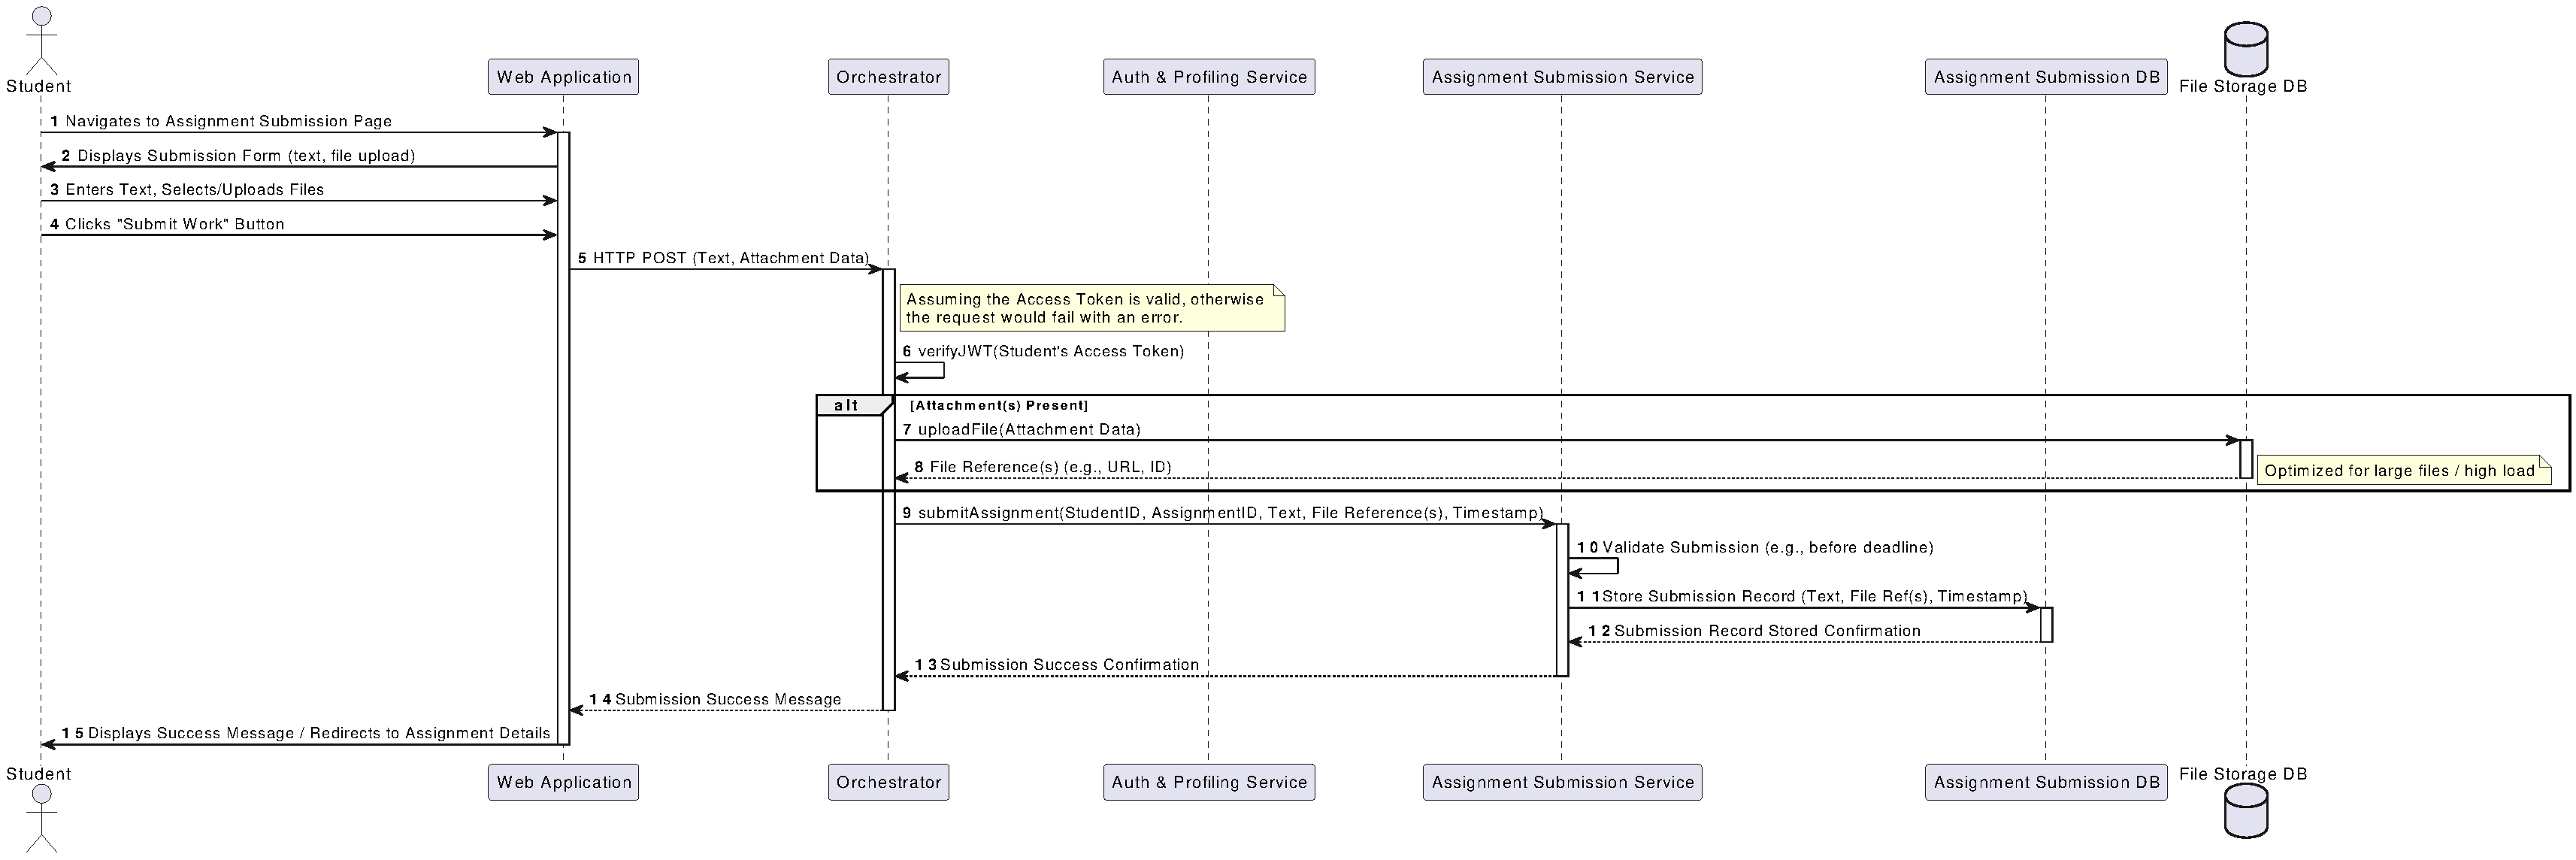
\includegraphics[width=0.9\linewidth]{Architettura/imgs/assign_submission_seq.pdf}
    \caption{Sequence diagram of the assignment submission process.}
    \label{fig:seqAssignmentSubmission}
\end{figure}

\subsection{Rationale}

\begin{justify}
    The design of the "Assignment Submission Flow" is optimized to address the critical \req{QA-PE-3}: Submission Peak requirement, which requires the system to be capable of handling a "large number of students (e.g., 100,000) attempting to submit their assignments concurrently". Therefore, the chosen architecture focuses on high throughput, low error rates, and efficient resource utilization, especially for file attachments.
\end{justify}
\begin{itemize}
    \item \textbf{Optimized File Handling for High Loads:}
    \begin{itemize}
        \item The \hyperref[def:Orchestrator]{Orchestrator}'s direct interaction with the FileStorageDB for attachment uploads is a design choice taken to bypass the \hyperref[def:AssignmentSubmissionService]{Assignment Submission Service} from the high load of processing large file streams. This approach ensures that the \hyperref[def:AssignmentSubmissionService]{Assignment Submission Service} handles lighter metadata (submission text, file references), allowing it to process a significantly higher volume of submission records efficiently, meeting the "All submission requests are successfully processed within 1 minute of reception" and "The error rate for submissions remains below 0.01\%" goals.
        \item By assigning file storage to a dedicated and scalable FileStorageDB, resources are utilized by the component best suited for the task. This helps maintain the "average CPU utilization of service instances does not exceed 80\% for more than 5 consecutive minutes".
        \item The \hyperref[def:AssignmentSubmissionService]{Assignment Submission Service} still exposes an interface that accepts files, though it’s not used in this scenario. This is compliant with the microservices architecture philosophy.
    \end{itemize}
    \item \textbf{Clear Separation of Concerns (Submission vs. File Storage):}
    \begin{itemize}
        \item In this case, the \hyperref[def:AssignmentSubmissionService]{Assignment Submission Service} focuses solely on managing records of submissions including information like who submitted what, when, and its status, along with references to files. This ensures its business logic remains focused on submission validation and state management.
        \item The FileStorageDB is specialized for efficient and scalable storage and retrieval of arbitrary binary data.
    \end{itemize}
    \item \textbf{Authorization and Role Enforcement:}
    \begin{itemize}
        \item The \hyperref[def:Orchestrator]{Orchestrator} acts as a security gate, leveraging the IAuthorization interface of the \hyperref[def:AuthProfilingService]{Auth \& Profiling Service}. This ensures that only authenticated "Students" who are "involved in a specific assignment" can submit their work. This centralized authorization mechanism prevents unauthorized access and maintains data integrity.
    \end{itemize}
    \item \textbf{Transactional Integrity:}
    \begin{itemize}
        \item The flow implies that a submission is only considered complete once both the file is stored (and a reference obtained) AND the submission record is created in AssignSubmDB. This ensures consistency, even if the actual database operations are distributed.
    \end{itemize}
\end{itemize}


\clearpage

\section{Peer Review Start}

\begin{figure}[h]
    \centering
    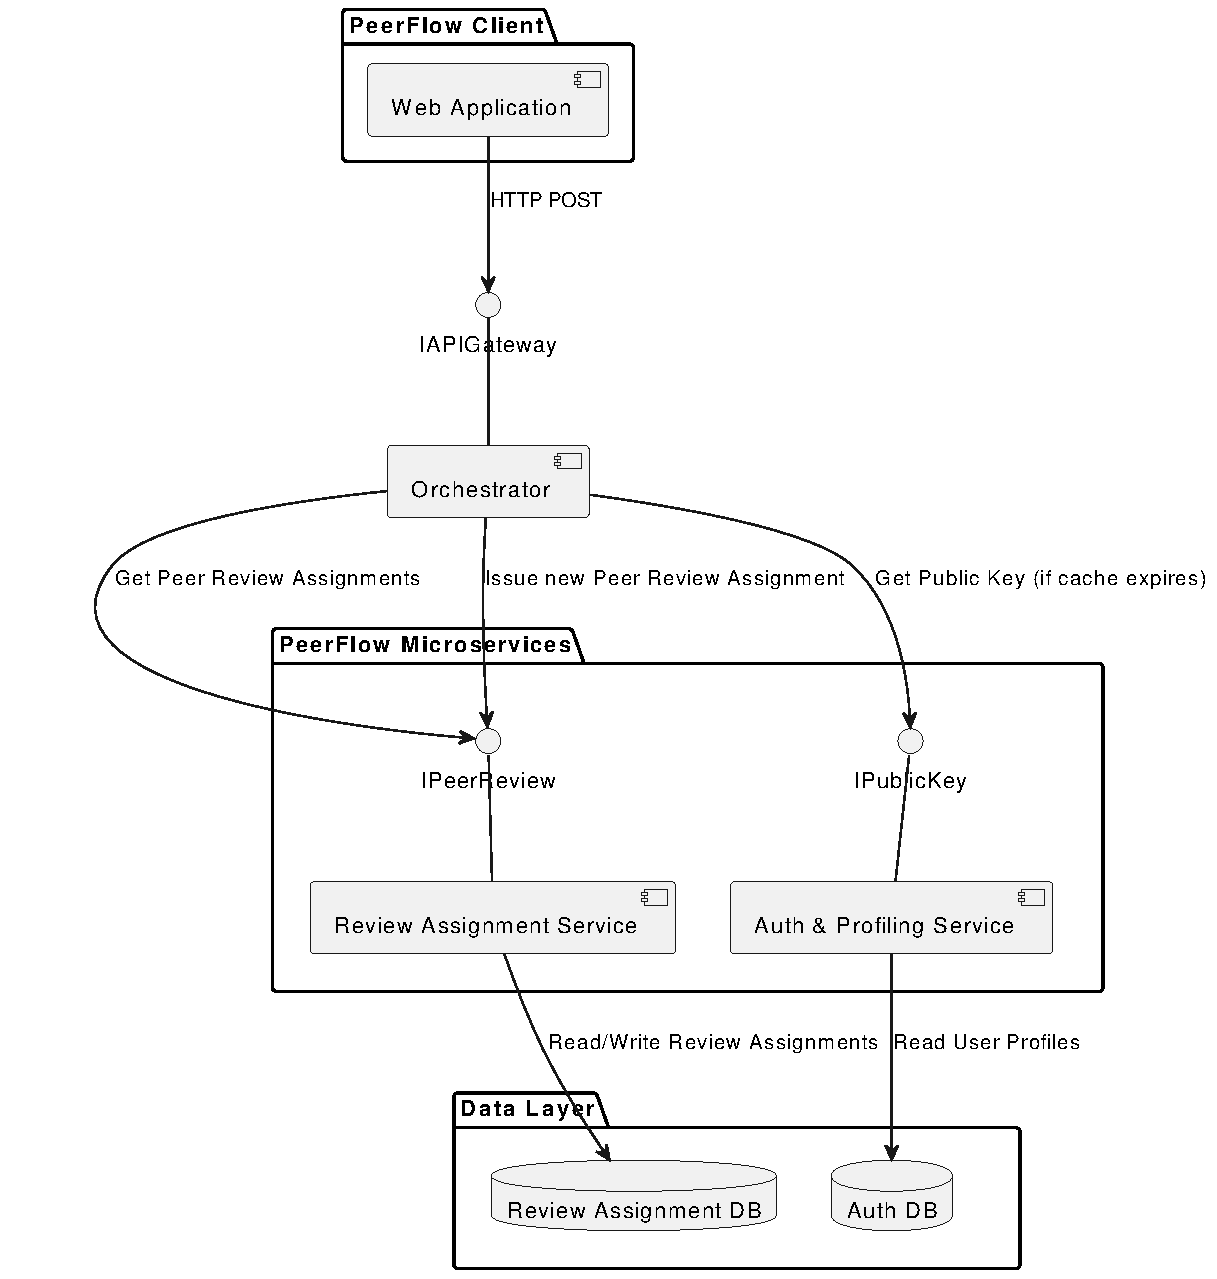
\includegraphics[width=0.7\linewidth]{Architettura/imgs/pr_start_cnc.pdf}
    \caption{C\&C view of the peer review start process.}
    \label{fig:ccPeerReviewStart}
\end{figure}
\clearpage

\subsection{Elements}

\begin{enumerate}
    \item \textbf{\hyperref[def:WebApplication]{Web Application}:} This is the client-side front-end application. It provides the user interface through which users can interact with the PeerFlow system’s microservices.
    \begin{itemize}
        \item \textbf{Peer Review Creation Form:} It shows the user a form which enables input for Rubric creation and Peer Review initialization. It also sends HTTP requests to the \hyperref[def:Orchestrator]{Orchestrator} to check assignment status, retrieve student lists (if manual pairing), define/edit/delete rubrics, and finally, to start the peer review process.
    \end{itemize}
    \item \textbf{\hyperref[def:Orchestrator]{Orchestrator} \hyperref[def:GenDetailsOrchestrator]{[General Details]}:} This service acts as the API Gateway for the PeerFlow system, coordinating the "Peer Review Start" flow.
    \begin{itemize}
        \item \textbf{Peer Reviews and Rubrics Management:} It forwards the requests related to peer reviews to the IPeerReview interface of the \hyperref[def:ReviewAssignmentService]{Review Assignment Service}. It also checks for correct review pairings.
        \item \textbf{Notification Trigger:} Upon successful initiation of the peer review process, it triggers notifications via the INotification interface of the \hyperref[def:NotificationService]{Notification Service} to inform students that they have been assigned peer reviews.
    \end{itemize}
    \item \textbf{\hyperref[def:AuthProfilingService]{Auth \& Profiling Service} \hyperref[def:GenDetailsAuth]{[General Details]}:} This microservice is responsible for user authentication and profile management.
    
    \item \textbf{\hyperref[def:ReviewAssignmentService]{Review Assignment Service}:} This microservice is central to managing the peer review phase.
    \begin{itemize}
        \item \textbf{IPeerReview interface - Peer Review creation:} It receives requests from the \hyperref[def:Orchestrator]{Orchestrator} to initiate a peer review. This includes setting the number of reviewers, confirming the rubric, specify the pairings.

         \item \textbf{Review Assignment DB:} This is the dedicated database instance for the \hyperref[def:ReviewAssignmentService]{Review Assignment Service}. It stores defined assessment rubrics (criteria, descriptions, scoring ranges) and the peer review assignment pairings (which student reviews which submission).
    \end{itemize}
   
    \item \textbf{\hyperref[def:NotificationService]{Notification Service} \hyperref[def:GenDetailsNotification]{[General Details]}:} This service exposes a REST API that allows to send email notifications to the users of the system.
    
    \item \textbf{Other Services \hyperref[def:GenDetailsOtherServices]{[General Details]}:} This aggregated component represents domain-specific microservices within the PeerFlow system that are not specifically relevant in the view.
\end{enumerate}

\clearpage
\subsection{Sequence Diagram}

\begin{figure}[h]
    \centering
    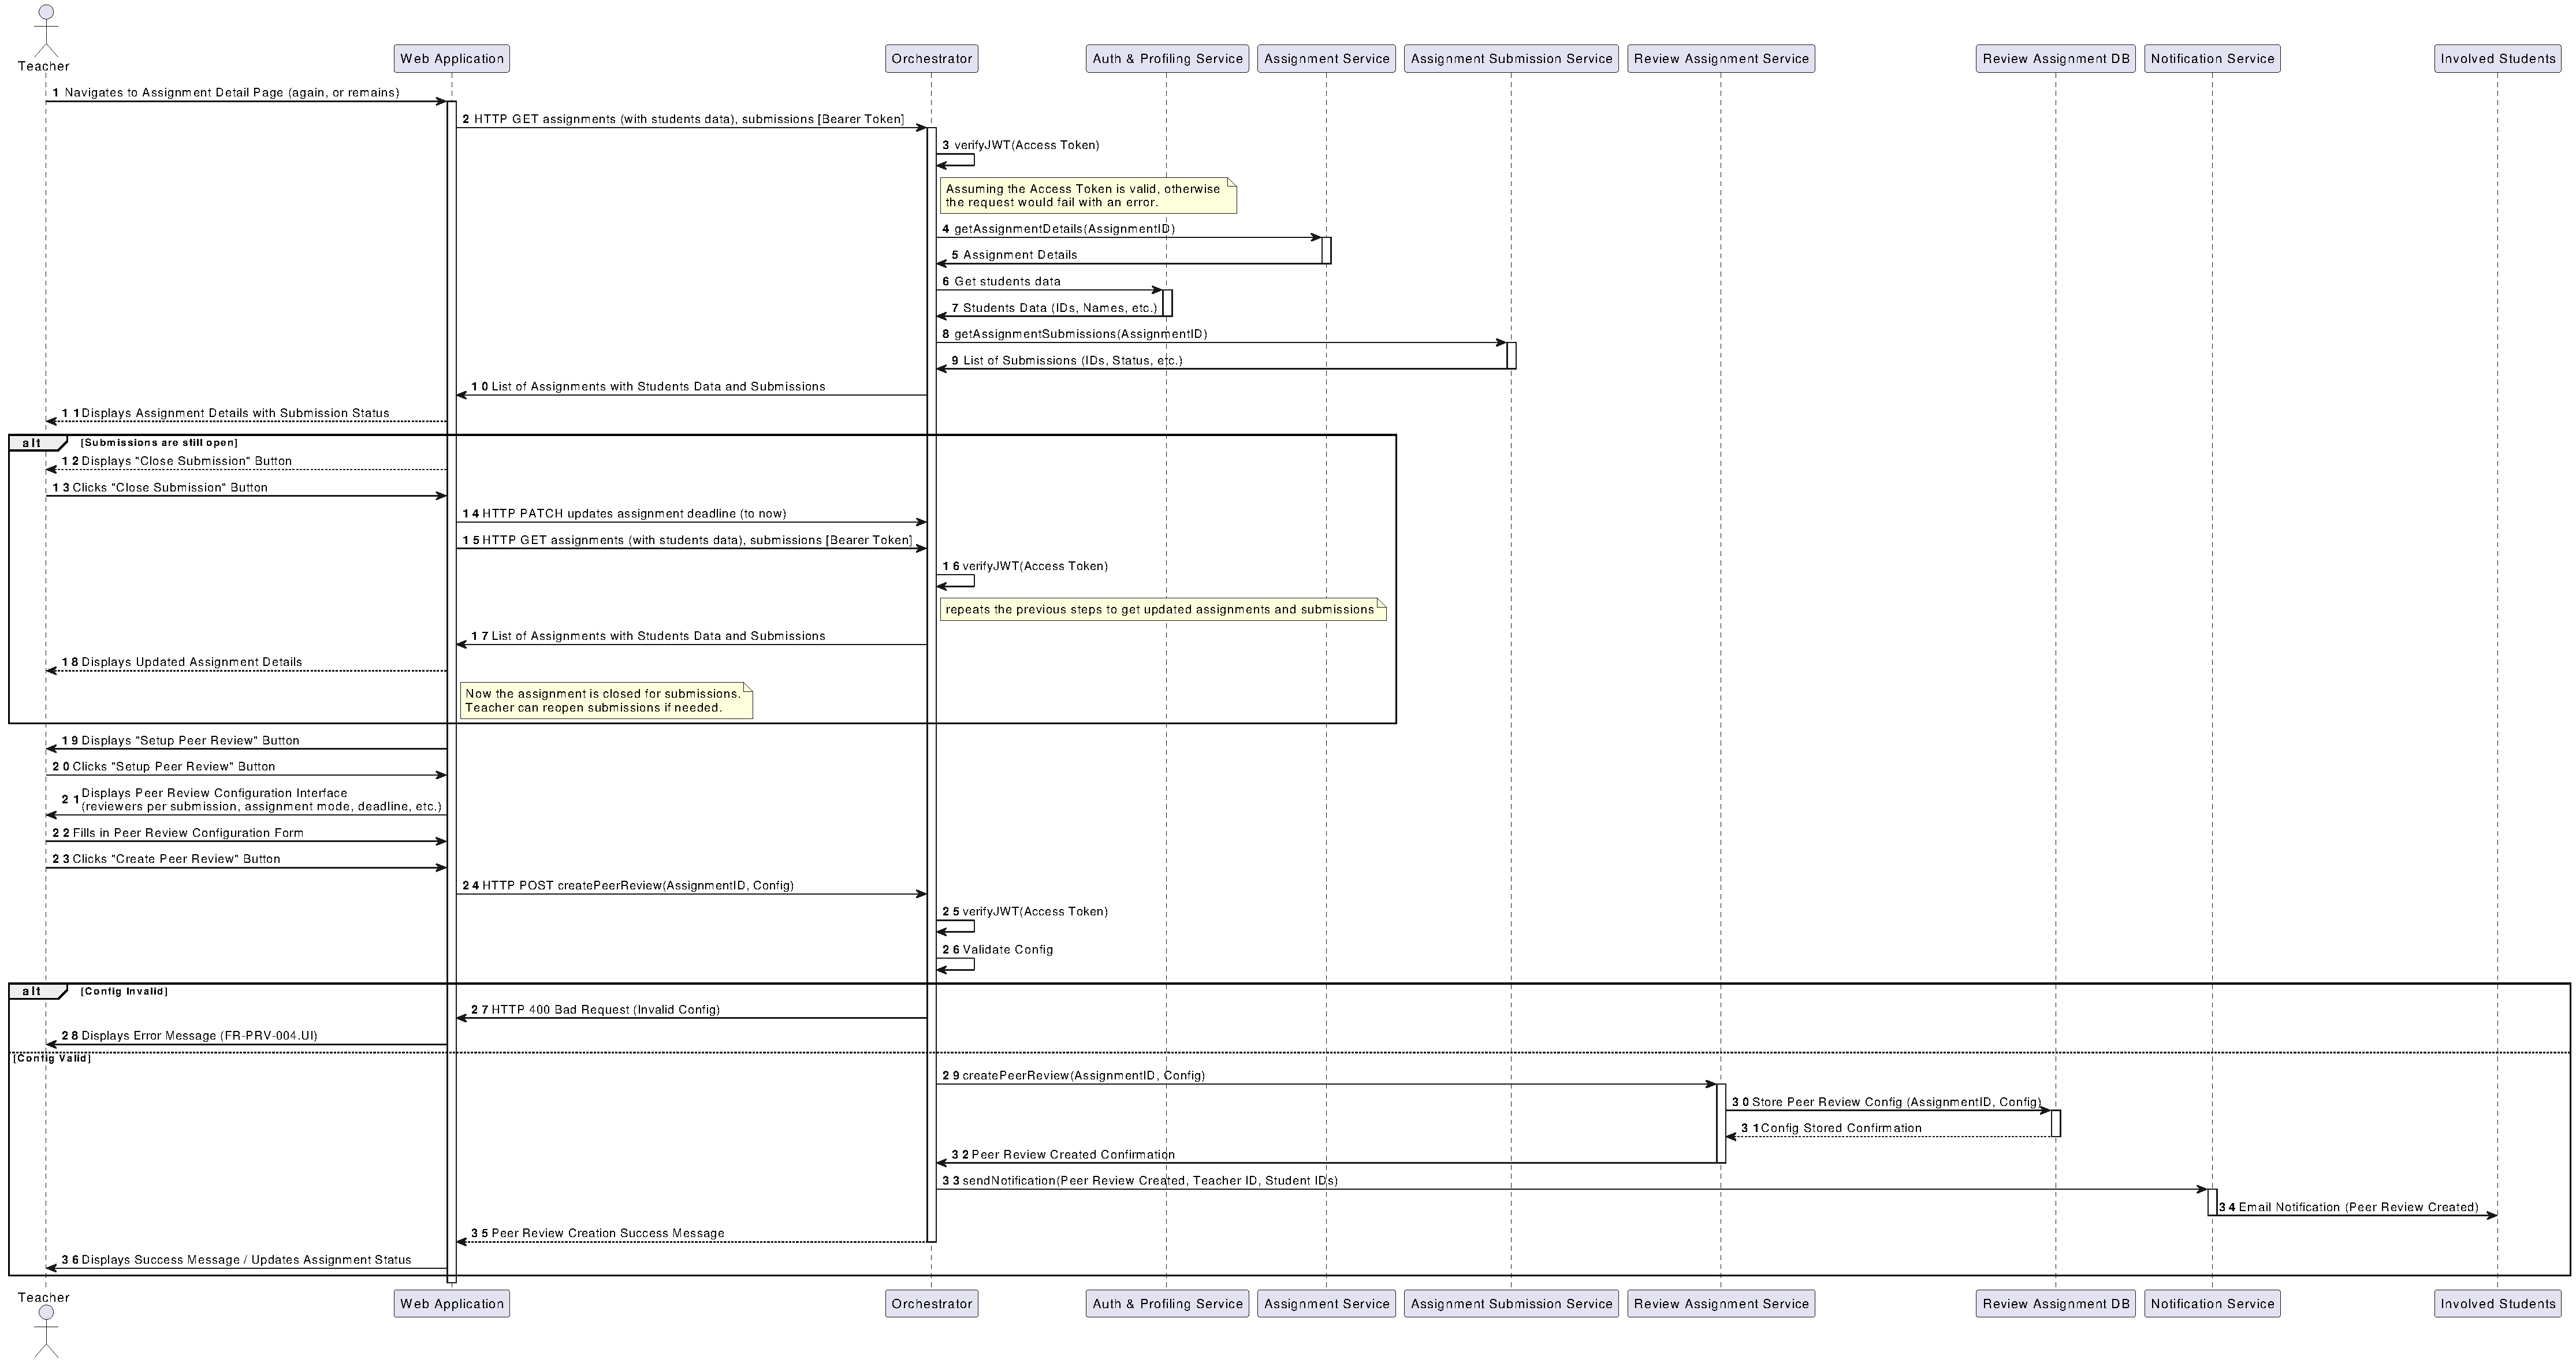
\includegraphics[width=0.9\linewidth]{Architettura/imgs/pr_start_seq.pdf}
    \caption{Sequence diagram of the peer review start process.}
    \label{fig:seqPeerReviewStart}
\end{figure}

\subsection{Rationale}

\begin{justify}
    The "Peer Review Start" flow is designed to provide teachers with flexible, secure, and reliable means to configure and initiate the peer evaluation process.
\end{justify}
\begin{itemize}
    \item \textbf{Teacher Role Enforcement and Authorization:}
    \begin{itemize}
        \item The \hyperref[def:Orchestrator]{Orchestrator} serves as a control point, performing JWT verification and role confirmation. This ensures security and prevents unauthorized modifications to assignments or review processes.
        
        \item The \hyperref[def:AuthProfilingService]{Auth \& Profiling Service} is the single source of truth for user roles and permissions. 
    \end{itemize}
    \item \textbf{Conditional Process Flow and Validation:}
    \begin{itemize}
        \item The system ensures that the preconditions for starting peer review are met. 
    \end{itemize}
    \item \textbf{Flexible Peer Review Assignment Mechanisms:}
    \begin{itemize}
        \item The system supports both "automatic (random)" and "manual (defined by the teacher)" peer assignment.
        \item The \hyperref[def:Orchestrator]{Orchestrator} initially fetches data of students, then, when a new Peer Review is being created, it checks for conditions: no students can review their own submission, the number of reviewers per assignment submission must be exactly the one specified by the teacher.
    \end{itemize}
    \item \textbf{Decoupled Notification for Students:}
    \begin{itemize}
        \item After peer reviews are assigned, students are notified via email.
        \item The \hyperref[def:Orchestrator]{Orchestrator} triggers this notification through the INotification interface of the \hyperref[def:NotificationService]{Notification Service}. This separation of concerns ensures that the core peer assignment logic in \hyperref[def:ReviewAssignmentService]{Review Assignment Service} is decoupled from the communication mechanism.
    \end{itemize}
    \item \textbf{Data Integrity and State Management:}
    \begin{itemize}
        \item The Review Assignment DB is dedicated to storing rubrics and peer review records, ensuring data autonomy and consistency for this critical phase.
    \end{itemize}
\end{itemize}


\clearpage
\section{Peer Review Submission}

\begin{figure}[h]
    \centering
    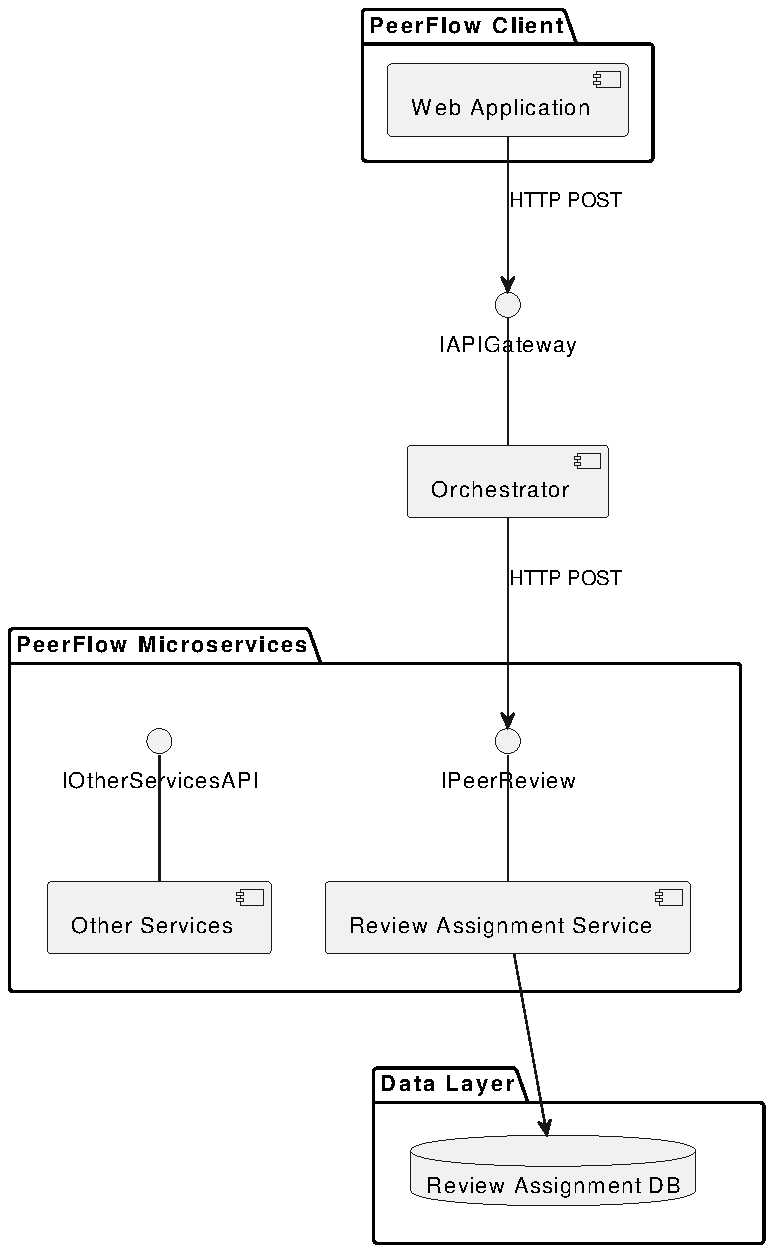
\includegraphics[width=0.5\linewidth]{Architettura/imgs/pr_subm_cnc.pdf}
    \caption{C\&C view of the peer review submission process.}
    \label{fig:ccPeerReviewSubmission}
\end{figure}
\clearpage

\subsection{Elements}

\begin{enumerate}
     \item \textbf{\hyperref[def:WebApplication]{Web Application}:} This is the client-side front-end application. It provides the user interface through which users can interact with the PeerFlow system’s microservices.
    \begin{itemize}
        \item \textbf{Peer Review Submission Form:} It shows a submission interface for a Peer Review, allowing students to view the submission they are reviewing and to input scores and feedback for each criterion. Also, displays the data of the submission under review.
    \end{itemize}
    
    \item \textbf{\hyperref[def:Orchestrator]{Orchestrator} \hyperref[def:GenDetailsOrchestrator]{[General Details]}:} This service acts as the API Gateway for the PeerFlow system, coordinating the "Peer Review Start" flow.

    \item \textbf{\hyperref[def:AuthProfilingService]{Auth \& Profiling Service} \hyperref[def:GenDetailsAuth]{[General Details]}:} This microservice is responsible for user authentication and profile management.
    
    \item \textbf{\hyperref[def:ReviewAssignmentService]{Review Assignment Service}:} This microservice is central to managing the peer review phase, including the assignment pairings, rubrics, and now, the processing and storage of completed reviews.
    \begin{itemize}
        \item \textbf{IPeerReview interface - Peer Review Submission:} It receives data from the \hyperref[def:Orchestrator]{Orchestrator} and registers the Peer Review in DB.
    
        \item \textbf{Review Assignment DB:} This is the dedicated database instance for the \hyperref[def:ReviewAssignmentService]{Review Assignment Service}. It stores peer review assignment pairings (which student reviews which submission), the assessment rubrics, and now also the completed peer review records (scores, textual justifications, reviewer identity, original author, timestamp).
    \end{itemize}
    
    \item \textbf{Other Services \hyperref[def:GenDetailsOtherServices]{[General Details]}:} This aggregated component represents domain-specific microservices within the PeerFlow system that are not specifically relevant in the view.
    
    \item \textbf{\hyperref[def:FileStorageService]{File Storage DB}:} This represents the underlying storage mechanism for file attachments. In this workflow, the \hyperref[def:Orchestrator]{Orchestrator} directly interacts with it to download files. 
\end{enumerate}

\clearpage
\subsection{Sequence Diagram}

\begin{figure}[h]
    \centering
    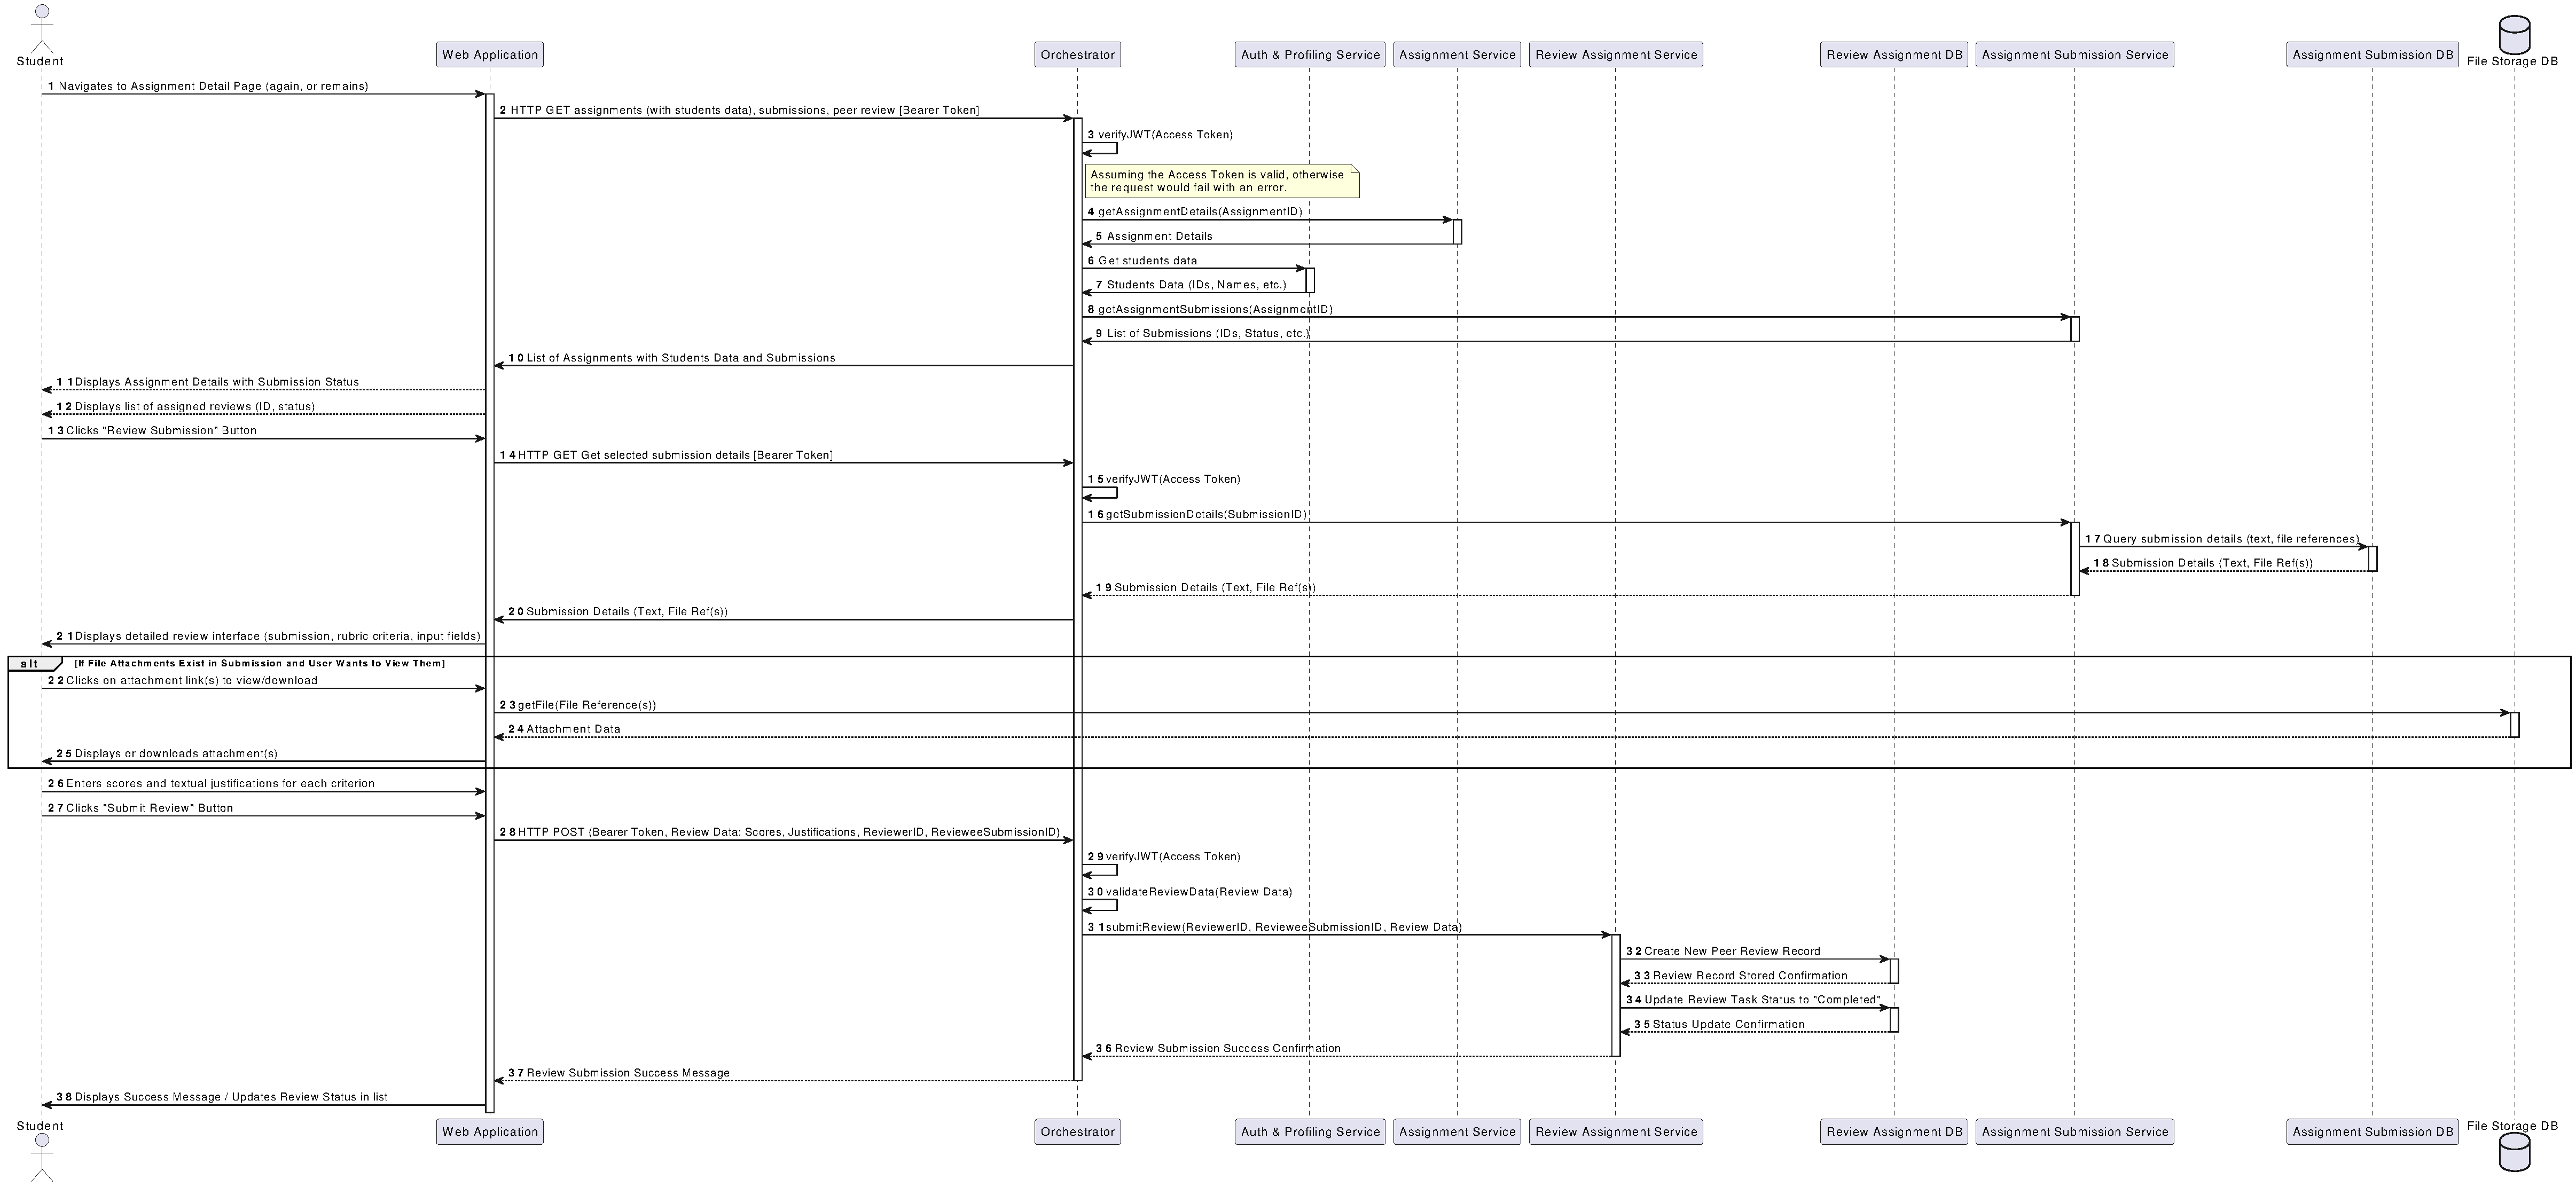
\includegraphics[width=0.9\linewidth]{Architettura/imgs/pr_subm_seq.pdf}
    \caption{Sequence diagram of the peer review submission process.}
    \label{fig:seqPeerReviewSubmission}
\end{figure}

\subsection{Rationale}

\begin{itemize}
    \item \textbf{Student Interface:}
    \begin{itemize}
        \item The flow begins with the \hyperref[def:WebApplication]{Web Application} displaying a list of assigned reviews to the student. When a student selects a submission, the \hyperref[def:WebApplication]{Web Application} presents a detailed review interface including the peer's submitted text and attachments. This ensures students have all the necessary information to conduct a good review.
    \end{itemize}
    \item \textbf{\hyperref[def:Orchestrator]{Orchestrator} as Intelligent Coordinator:}
    \begin{itemize}
        \item The \hyperref[def:Orchestrator]{Orchestrator} acts as the coordinator for all interactions between the \hyperref[def:WebApplication]{Web Application} and the other services involved. This simplifies the client-side logic, as the \hyperref[def:WebApplication]{Web Application} only communicates with one API Gateway (IAPIGateway).
        \item \textbf{Authorization Enforcement:} At every step, the \hyperref[def:Orchestrator]{Orchestrator} performs authorization checks. This ensures that only authenticated students can access their assigned reviews and that they are reviewers for that specific submission.
        
        \item \textbf{Data Aggregation for UI:} The \hyperref[def:Orchestrator]{Orchestrator} is responsible for aggregating data from multiple microservices before presenting it to the \hyperref[def:WebApplication]{Web Application}. This offloads complexity from the frontend and ensures a coherent data model for display.
        
        \item \textbf{File Retrieval:} The \hyperref[def:WebApplication]{Web Application} retrieves file attachments from the \hyperref[def:FileStorageService]{File Storage DB} using references obtained from the \hyperref[def:AssignmentSubmissionService]{Assignment Submission Service}. This pattern is efficient for handling large files, ensuring that the \hyperref[def:AssignmentSubmissionService]{Assignment Submission Service} only handles metadata and doesn't become a bottleneck for data transfer.
    \end{itemize}
    \item \textbf{Dedicated Services for Core Responsibilities:}
    \begin{itemize}
        \item \textbf{\hyperref[def:ReviewAssignmentService]{Review Assignment Service} for Review Data Management:} This service manages review assignments, rubrics, and also the processing and storage of completed peer review records. It provides interfaces that encapsulate all review-specific business logic. Validations like checking scores against rubric ranges and requiring justifications are performed here.
        
        \item \textbf{\hyperref[def:AssignmentSubmissionService]{Assignment Submission Service} for Submission Content:} This service remains the authoritative source for the content of student submissions (text and file references). This separation maintains a clear boundary between the "submission" and "review" domains, addressing the separation of concerns principle.
        
        \item \textbf{\hyperref[def:FileStorageService]{File Storage DB} for Efficient File Access:} Its direct interaction with the \hyperref[def:Orchestrator]{Orchestrator} for \texttt{getFile()} calls ensures fast and scalable retrieval of attachments.
    \end{itemize}
    \item \textbf{Data Integrity and State Management:}
    \begin{itemize}
        \item The Review Assignment DB is the single source for peer review assignments, rubrics, and the completed review records. This ensures consistency across the system regarding the status and content of reviews.
    \end{itemize}
\end{itemize}

\clearpage
\section{Peer Review Results Aggregation}

\begin{figure}[h]
    \centering
    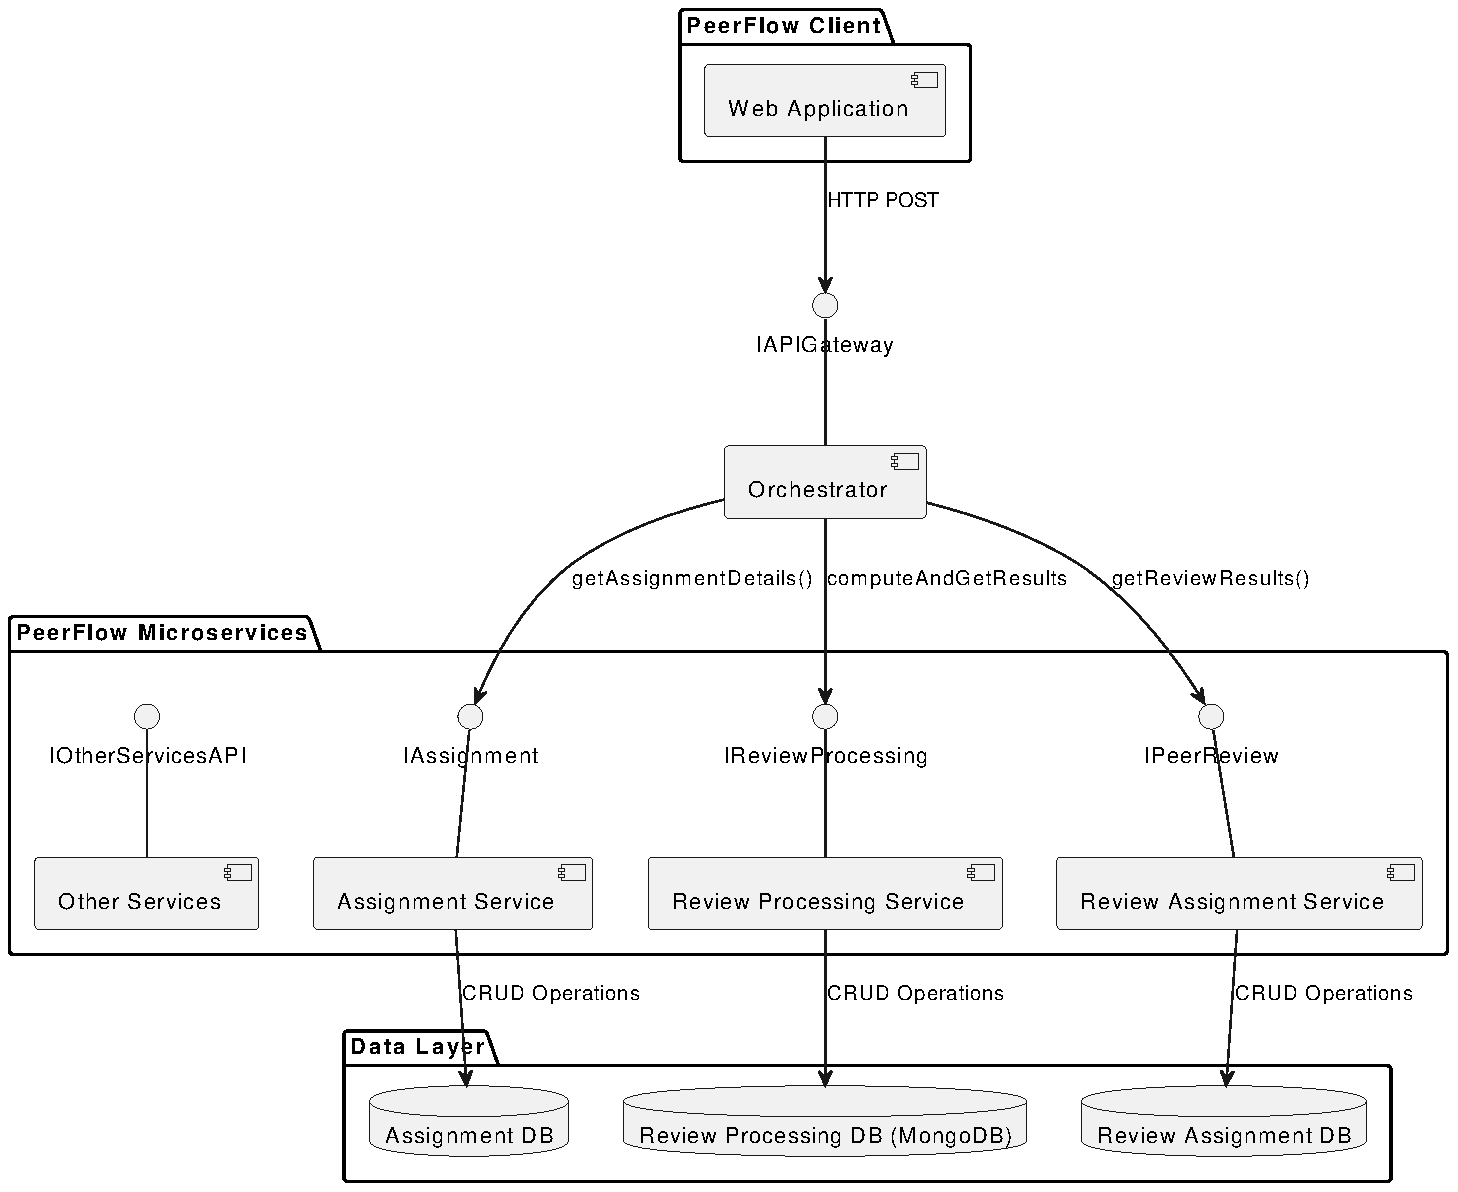
\includegraphics[width=0.9\linewidth]{Architettura/imgs/pr_proc_cnc.pdf}
    \caption{C\&C view of the peer review results aggregation process.}
    \label{fig:ccPeerReviewResultsAggregation}
\end{figure}
\clearpage

\subsection{Elements}

\begin{enumerate}
    \item \textbf{\hyperref[def:WebApplication]{Web Application}:} This is the client-side front-end application. It provides the user interface through which users can interact with the PeerFlow system’s microservices.
    \begin{itemize}
        \item \textbf{Start Aggregation Button:} The \hyperref[def:WebApplication]{Web Application} presents the teacher with a button to manually initiate the review aggregation process for a specific assignment. It sends the HTTP \texttt{POST} request to the \hyperref[def:Orchestrator]{Orchestrator} when the teacher triggers the aggregation.
    \end{itemize}
    
    \item \textbf{\hyperref[def:Orchestrator]{Orchestrator} \hyperref[def:GenDetailsOrchestrator]{[General Details]}:} This service acts as the API Gateway for the PeerFlow system, coordinating the "Peer Review Start" flow.
    \begin{itemize}
        \item \textbf{Data Extraction Orchestration:} Instead of the \hyperref[def:ReviewProcessingService]{Review Processing Service} extracting data directly, the \hyperref[def:Orchestrator]{Orchestrator} now orchestrates the extraction. It calls the IAssignment interface of the \hyperref[def:AssignmentService]{Assignment Service} and the IPeerReview interface of the \hyperref[def:ReviewAssignmentService]{Review Assignment Service} to check that the requesting teacher is the creator of the assignment and to gather all the necessary raw data (completed reviews, rubrics, and pairings) for the specific assignment.
        
        \item \textbf{Aggregation Trigger:} After extracting the raw data, the \hyperref[def:Orchestrator]{Orchestrator} calls the IReviewProcessing interface of the \hyperref[def:ReviewProcessingService]{Review Processing Service}, passing this extracted raw review data to it to initiate the aggregation calculation.
    \end{itemize}
    \item \textbf{\hyperref[def:ReviewAssignmentService]{Review Assignment Service}:} This microservice is responsible for managing peer review assignments, rubrics, and storing the raw, individual completed review records submitted by students.
    \begin{itemize}
        \item \textbf{IPeerReview interface - Raw Data Provider:} It provides the essential interfaces that the \hyperref[def:Orchestrator]{Orchestrator} (now acting as the extractor) uses to retrieve the necessary raw data for aggregation.
        
        \item \textbf{Review Assignment DB:} This is the dedicated database instance for the \hyperref[def:ReviewAssignmentService]{Review Assignment Service}. It serves as the source of raw data for the aggregation process, storing individual completed peer review records, the assessment rubrics, and the peer review assignment pairings. 
    \end{itemize}
    
    \item \textbf{\hyperref[def:ReviewProcessingService]{Review Processing Service}:} This is the dedicated microservice performing the ETL (Extract, Transform, Load) process for peer review results. Its core function is to compute and store aggregated statistics from the raw review data.
    \begin{itemize}
        \item \textbf{IPeerReview interface - Aggregation Initiation:} It receives the raw review data (extracted by the \hyperref[def:Orchestrator]{Orchestrator}) and executes the calculation.
        
        \item \textbf{Transformation:} It performs the analytics and calculations to derive the aggregated results (e.g., overall average scores, per-criterion averages, score distributions for assignments, and aggregated scores/counts per submission and per reviewer) as defined by your AggregatedByAssignmentResult, AggregatedBySubmissionResult, and AggregatedByReviewResult data views.
        
        \item \textbf{Loading:} Once computed, it stores these aggregated results into its dedicated Review Processing DB (MongoDB).

        \item \textbf{Review Processing DB:} This is the dedicated database instance for the \hyperref[def:ReviewProcessingService]{Review Processing Service}, explicitly identified as MongoDB to suit the flexible and analytical nature of aggregated results. It stores the pre-computed, aggregated results: AggregatedByAssignmentResult, AggregatedBySubmissionResult, and AggregatedByReviewResult objects. These are optimized for fast querying and reporting.
    \end{itemize}
    
    \item \textbf{\hyperref[def:AssignmentService]{Assignment Service}:} This microservice manages assignment details, including their status.
    \begin{itemize}
        \item \textbf{IAssignment interface - Status Update:} The \hyperref[def:Orchestrator]{Orchestrator} uses this interface to retrieve all necessary assignment data.

        \item \textbf{Assignment DB:} This is the dedicated database instance for the \hyperref[def:AssignmentService]{Assignment Service}. It stores assignment details.
    \end{itemize}
    
    \item \textbf{Other Services \hyperref[def:GenDetailsOtherServices]{[General Details]}:} This aggregated component represents domain-specific microservices within the PeerFlow system that are not specifically relevant in the view.
\end{enumerate}

\subsection{Sequence Diagram}

\begin{figure}[h]
    \centering
    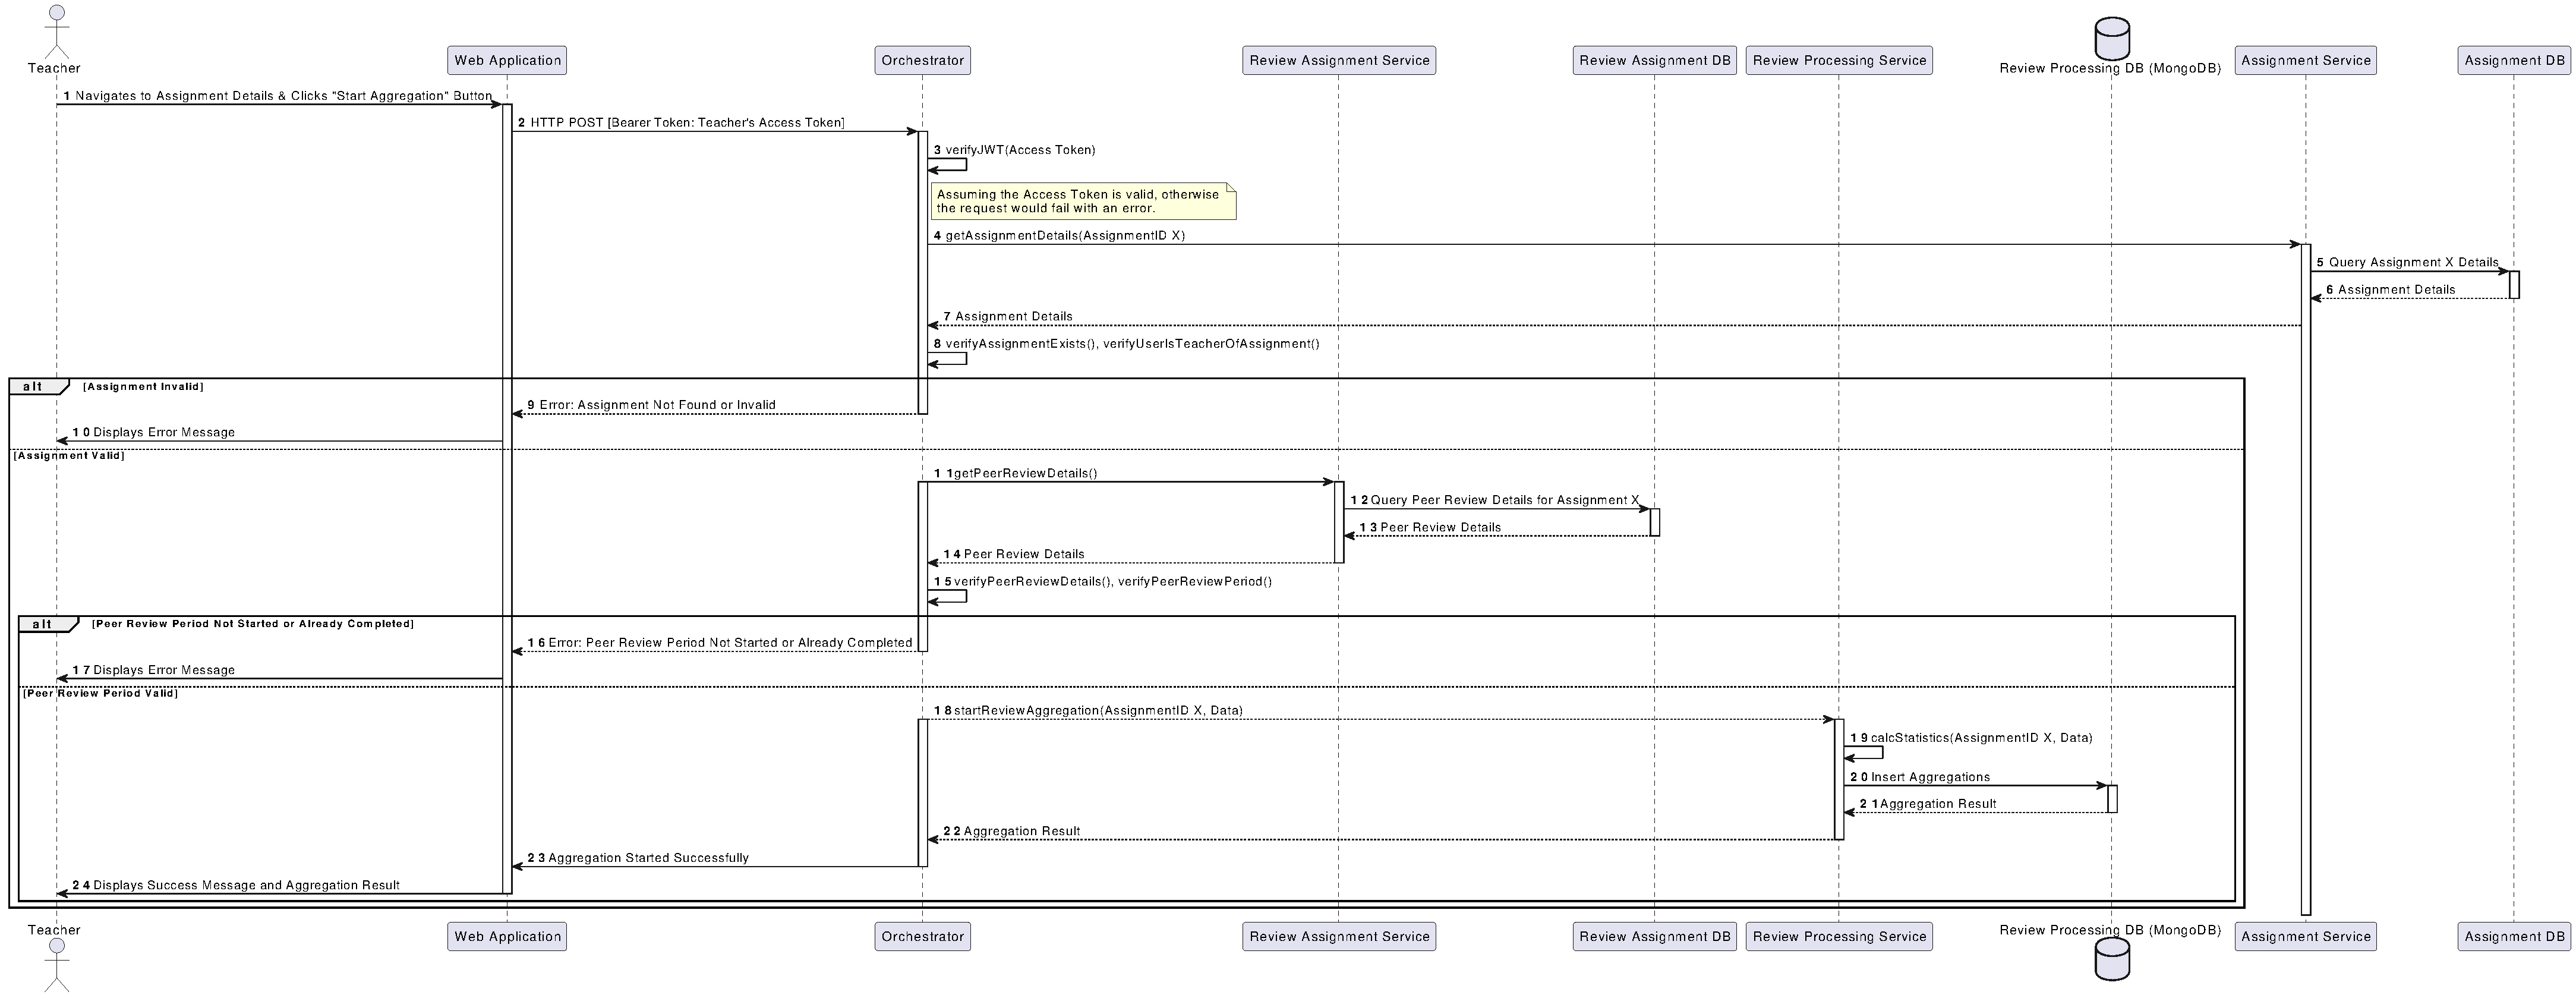
\includegraphics[width=0.9\linewidth]{Architettura/imgs/pr_proc_seq.pdf}
    \caption{Sequence Diagram of the peer review results aggregation process.}
    \label{fig:seqPeerReviewResultsAggregation}
\end{figure}

\subsection{Rationale}

\begin{justify}
    The "Peer Review Results Aggregation Flow" is designed as a distinct ETL (Extract, Transform, Load) process, addressing the requirements for "Aggregation and visualization of evaluation results for students and teachers" and "Accessing detailed evaluation reports for teachers". 
\end{justify}
\begin{itemize}
    \item \textbf{Teacher-Initiated Processing:}
    \begin{itemize}
        \item Teachers are in direct control over when aggregation occurs, allowing them to finalize reviews and verify conditions before results are processed and released.
        \item The \hyperref[def:WebApplication]{Web Application} exposes a "Start Aggregation" button, which sends a request to the \hyperref[def:Orchestrator]{Orchestrator}.
    \end{itemize}
    \item \textbf{\hyperref[def:Orchestrator]{Orchestrator} as Coordinator:}
    \begin{itemize}
        \item The \hyperref[def:Orchestrator]{Orchestrator} acts as the central coordinator, bridging the \hyperref[def:WebApplication]{Web Application} with the backend services for aggregation.
        
        \item \textbf{Authorization:} It first authorizes the teacher's request, verifying their JWT token and role to ensure only authorized teachers can initiate this process for their assignments.
        
        \item \textbf{Data Extraction:} Crucially, the \hyperref[def:Orchestrator]{Orchestrator} now takes direct responsibility for extracting all necessary raw data from the \hyperref[def:ReviewAssignmentService]{Review Assignment Service}. It calls IPeerReview to retrieve completed reviews, rubric details, and peer review pairings. This consolidates data retrieval logic at the API Gateway level.
        
        \item \textbf{Aggregation Trigger:} After successfully extracting the raw data, the \hyperref[def:Orchestrator]{Orchestrator} then explicitly triggers the \hyperref[def:ReviewProcessingService]{Review Processing Service} (IReviewProcessing), passing the extracted raw data to it. This design ensures that the \hyperref[def:ReviewProcessingService]{Review Processing Service} receives precisely the data it needs to perform its calculations.
    \end{itemize}
    \item \textbf{\hyperref[def:ReviewAssignmentService]{Review Assignment Service} as Authoritative Raw Data Source:}
    \begin{itemize}
        \item \hyperref[def:ReviewAssignmentService]{Review Assignment Service} remains the single source for all raw review-related data: individual completed reviews, assessment rubrics, and the peer review assignment pairings.
        \item The \hyperref[def:Orchestrator]{Orchestrator} explicitly reads this data from \hyperref[def:ReviewAssignmentService]{Review Assignment Service}'s interfaces, ensuring consistency and preventing redundant data storage elsewhere. This aligns with the microservices principle of data ownership.
    \end{itemize}
    \item \textbf{\hyperref[def:ReviewProcessingService]{Review Processing Service} for Dedicated Analytical Processing:}
    \begin{itemize}
        \item The role of the \hyperref[def:ReviewProcessingService]{Review Processing Service} is highly specialized: it performs the calculation of statistics ("Transform" phase) and stores the results in its database ("Load" phase).
        \item By receiving pre-extracted data from the \hyperref[def:Orchestrator]{Orchestrator}, the \hyperref[def:ReviewProcessingService]{Review Processing Service} can focus on its analytical task, which is optimized for fast read access for reporting.
        \item The use of Review Processing DB (MongoDB) is ideal for storing flexible, aggregated analytical results, enabling fast querying for visualization.
    \end{itemize}
\end{itemize}